\documentclass[12pt]{report}
\usepackage{graphicx} % Required for inserting images
\usepackage{subcaption}
\usepackage{cmap}
\usepackage[T1]{fontenc}
\usepackage{lmodern}
\usepackage{microtype}
\usepackage{setspace}
\onehalfspacing
% \usepackage{polski}
\usepackage{geometry}
\usepackage{amsmath,amssymb,amsfonts}
\usepackage{siunitx}
\usepackage{booktabs}
\sisetup{per-mode=fraction, inter-unit-product =\ensuremath{{}\cdot{}}}
\usepackage{tikz}
\usetikzlibrary{arrows.meta, decorations.pathmorphing}
\usepackage{tikzducks}
% \usepackage{twemojis}
\usepackage[backend=biber,style=numeric,sorting=none,maxnames=6,url=false,doi=true,isbn=false,giveninits=true]{biblatex}
\addbibresource{lio.bib}
\usepackage{indentfirst}
\setlength{\marginparwidth}{4cm}
\setlength{\marginparsep}{0.5cm}
\usepackage[figwidth=0.75\textwidth,figcolor=black!20,disable]{todonotes}
\usepackage{marginnote}
\let\marginpar\marginnote % https://tex.stackexchange.com/a/631449


\usepackage{xcolor}
\usepackage[normalem]{ulem}

\usepackage{fancyhdr}
\pagestyle{fancy}
\fancyhf{}
\fancyhead[L]{\nouppercase{\leftmark}}
\fancyhead[R]{\thepage}
\renewcommand{\chaptermark}[1]{\markboth{\thechapter.\ #1}{}}
\renewcommand{\headrulewidth}{0.4pt}
\setlength{\headheight}{15pt}

% Chapter-opening pages use the ``plain'' style: show only the page number
% because the chapter title is already printed on the page.
\fancypagestyle{plain}{%
    \fancyhf{}%
    \fancyhead[R]{\thepage}%
    \renewcommand{\headrulewidth}{0pt}%
}

% Page number only, used for standalone declarations.
\fancypagestyle{numberonly}{%
    \fancyhf{}%
    \fancyhead[R]{\thepage}%
    \renewcommand{\headrulewidth}{0pt}%
}

\makeatletter
\newcommand{\chapterduck}{%
    \begin{tikzpicture}[scale=0.52,baseline=(current bounding box.south)]
        \ifcase\value{chapter}
            \duck[graduate,book={Thesis}]
        \or
            \duck[bobblehat=red!70!black,
            % book={Ps},bookcolour=blue!60!black,
            shovel=gray
            ]
        \or
            \duck[glasses, viking,
            % book={$\Delta\phi$},bookcolour=violet!70!black,
            magicwand
            ]
        \or
            \duck[squareglasses,think={?},bubblecolour=blue!10]
        \or
            \duck[graduate,signpost={!},signback=green!50!black]
        \else
            \duck[graduate,book={Thesis}]
        \fi
    \end{tikzpicture}%
}
\renewcommand{\@makechapterhead}[1]{%
    \vspace*{12pt}%
    {\parindent\z@\raggedright\normalfont
        \ifnum\c@secnumdepth>\m@ne
            {\noindent\large\scshape\textls[100]{\@chapapp\ \thechapter}\par}%
            \vspace{4pt}%
            \noindent\makebox[\textwidth][l]{%
                \rule{\textwidth}{0.5pt}%
                \llap{\raisebox{1mm}[0pt][0pt]{\chapterduck}}%
            }\par
            \vspace{10pt}%
        \fi
        {\Huge\bfseries #1\par}%
        \vspace{28pt}%
    }%
}
\renewcommand{\@makeschapterhead}[1]{%
    \vspace*{12pt}%
    {\parindent\z@\raggedright\normalfont
        {\Huge\bfseries #1\par}%
        \vspace{6pt}%
        \rule{\textwidth}{0.5pt}\par
        \vspace{22pt}%
    }%
}
\makeatother

\usepackage{hyperref} % remember to keep it last

\title{thesis draft}
\author{Mateusz Winiarski}
\date{July 2026}

%TC:macro \todo [ignore]


\begin{document}
\setcounter{page}{1}
\newgeometry{left=2.0cm, top=2.0cm, bottom=2.0cm, right=2.0cm}
\thispagestyle{empty}
\begin{center}
\begin{figure}
    \centering
    
\includegraphics[width=0.15\linewidth]{uj.png}
\end{figure}
\vspace{-1cm}
           \Large
	\textbf{Jagiellonian University in Kraków}\vspace{0.2cm}\\ Faculty of Physics, Astronomy and Applied Computer Science
               \vspace*{1cm}
         \vspace{1cm}
         \Large
          \textbf{Mateusz Winiarski}\\\vspace{0.4cm}
         \normalsize Student ID no.: 1176241\\
             \vspace{1cm}
        \LARGE
        \textbf{Sensitivity Comparison of Atomic Interferometry and Deflectometry for Gravitational Measurements on Positronium Using Monte Carlo Simulations}
      
        \vspace{1.5cm}
        \normalsize
       Master's thesis in physics (path: experimental physics)\\ \vspace{0.15cm}
        
        \vfill
        \vspace{1.5cm}
       \begin{minipage}{1\textwidth}
\begin{flushright}
Thesis written under the supervision of\\
dr Sushil Sharma\\
Marian Smoluchowski Institute of Physics, JU
\end{flushright}
\end{minipage}
        
        \vspace{1.5cm}
        \begin{center}
      Kraków, 2026
        \end{center}
\end{center}

\clearpage
\thispagestyle{empty}
\vspace{2.5cm}
\begin{flushleft}
\large \textbf{Oświadczenie autora pracy / Thesis' author statement}\vspace{0.6cm}\\
\end{flushleft}

\noindent Świadom odpowiedzialności prawnej oświadczam, że niniejsza praca dyplomowa została napisana przeze mnie samodzielnie i nie zawiera treści uzyskanych w sposób niezgodny z obowiązującymi przepisami.

\noindent Oświadczam również, że przedstawiona praca nie była wcześniej przedmiotem procedur związanych z uzyskaniem tytułu zawodowego w wyższej uczelni.

\noindent Aware of legal responsibility, I hereby declare that this diploma thesis was written independently by me and does not include content obtained in a manner inconsistent with applicable law.

\noindent I also declare, that the presented thesis has not previously been the subject of procedures related to obtaining a professional title at an academic institution.
\vspace{2cm}
\begin{center}
\begin{tabular}{cc}
\makebox[7cm]{\hrulefill} & \makebox[7cm]{\hrulefill} \\
Kraków, dnia / Kraków, dated & Podpis autora pracy / Author signature
\end{tabular}
\end{center}
\vfill
\begin{flushleft}
\large \textbf{Oświadczenie kierującego pracą / Thesis' supervisor statement}
\end{flushleft}

\noindent Potwierdzam, że niniejsza praca została przygotowana pod moim kierunkiem i~kwalifikuje się do przedstawienia jej w postępowaniu o nadanie tytułu zawodowego.

\noindent I confirm that this thesis was prepared under my supervision and it qualifies to be presented in the proceedings for the granting of a professional title.
\vspace{2cm}
\begin{center}
\begin{tabular}{cc}
\makebox[7cm]{\hrulefill} & \makebox[7cm]{\hrulefill} \\
Kraków, dnia / Kraków, dated & Podpis kierującego pracą / Supervisor signature
\end{tabular}
\end{center}
\vfill

\clearpage
\thispagestyle{empty}
\begin{abstract}
% \large\textbf{Abstract}

%preliminary - check numbers
The weak equivalence principle has not been tested directly
on a purely leptonic matter--antimatter system. Positronium, the bound state of
an electron and a positron, provides such a system, and its metastable $2^3S$
state lives long enough to serve as a test particle for inertial sensing. The
feasibility of inertial sensing with a $2^3S$ positronium beam is investigated
through Monte Carlo simulations of two proposed schemes: a classical moir\'e
deflectometer and a Mach--Zehnder interferometer. The Monte Carlo model tracks
individual positronium atoms, assigning their velocities according to a velocity distribution based on measured $2^3S$ beam characteristics, an angular divergence in the milliradian range, and lifetimes sampled
from an exponential distribution. The acceleration is inferred from the displacement or phase shift of the periodic pattern measured with a third, scanning grating. For a mean velocity of $10^5~\mathrm{m/s}$ and acquisition time of 5.3 weeks the interferometer’s minimum detectable
acceleration is $(140 \pm 1)~\mathrm{m/s^2}$ (tens of times better than with
the deflectometer), in accord with the analytically predicted order. The
interferometer sensitivity is optimal at a beam divergence of about
$1.6~\mathrm{mrad}$ and remains within a broad, tolerant region of the
velocity--divergence plane. These results identify the interferometer as the
preferred scheme for a precise  gravitational measurement on positronium and
quantify the beam conditions required for such measurements.

\vfill

\textbf{Keywords}: positronium; antimatter gravity; Mach--Zehnder interferometer; moiré deflectometry; Monte Carlo simulations; inertial sensing.
\vfill
~
\end{abstract}


\clearpage
\thispagestyle{empty}
\renewcommand{\abstractname}{Streszczenie}
\begin{abstract}
% \large\textbf{Streszczenie}

Słaba zasada równoważności nie została dotąd zbadana bezpośrednio w układzie czysto leptonowym materia--antymateria. Pozytonium, stan związany elektronu i pozytonu, stanowi taki układ, a jego metastabilny stan $2^3S$ żyje wystarczająco długo, aby służyć jako cząstka testowa w pomiarach inercyjnych. Wykonalność pomiarów inercyjnych z użyciem wiązki pozytonium w stanie $2^3S$ analizowano za pomocą symulacji Monte Carlo dla dwóch proponowanych schematów: klasycznego deflektometru moir\'e oraz interferometru Macha--Zehndera. Model Monte Carlo śledzi pojedyncze atomy pozytonium, przypisując im prędkości zgodnie z rozkładem prędkości opartym na zmierzonych charakterystykach wiązki $2^3S$, rozbieżność kątową rzędu miliradianów oraz czas życia losowany z rozkładu wykładniczego. Przyspieszenie wyznacza się na podstawie przesunięcia okresowego wzoru bądź jego przesunięcia fazowego, mierzonych za pomocą trzeciej, skanującej siatki. Dla średniej prędkości $10^5$ \si{\metre\per\second} i czasu akwizycji 5,3 tygodnia minimalne wykrywalne przyspieszenie dla interferometru wynosi $(140\pm1)$ \si{\metre\per\second\squared} (kilkadziesiąt razy lepsze niż w przypadku deflektometru), zgodnie z przewidywanym analitycznie rzędem wielkości. Czułość interferometru jest największa dla rozbieżności kątowej wiązki około $1{,}6$ mrad i pozostaje wysoka w szerokim, tolerancyjnym obszarze płaszczyzny prędkość--rozbieżność. Wyniki te wskazują interferometr jako preferowany schemat do precyzyjnych pomiarów grawitacyjnych na pozytonium oraz określają ilościowo warunki, jakie musi spełniać wiązka pozytonium do przeprowadzenia takich pomiarów.
% \end{center}
\vfill

\textbf{Słowa kluczowe}: pozytonium; grawitacja antymaterii; interferometr Macha--Zehndera; deflektometria moir\'e; symulacje Monte Carlo; pomiary inercyjne.
\vspace{1cm}
~
\end{abstract}

\clearpage
\thispagestyle{empty}

\begin{center}
\vspace*{6cm}

{\Large\itshape
When I'm left home alone\\
I know all the explosions from Structure of Matter by heart\\
Once again, I've broken the entire internet\\
Suddenly, Nuclear Physics fell into my hands\\
I'll be calculating all night long\\[1em]
I'll draw nuclei all over my wall\\
But please, oh please, don't tell the Dean\par
}
\end{center}

\vspace{1cm}

\begin{flushright}
-- -- SMP (Studio of Music and Poetry), 'Nuclei on Wall'\\
{\footnotesize from the upcoming album 'Study Me Half'}
\end{flushright}

\restoregeometry
\setcounter{page}{6}
\clearpage
\tableofcontents

\clearpage

\clearpage
\listoffigures 

\clearpage
\listoftables  

% \newgeometry{right=5cm,marginparwidth=4cm,marginparsep=0.5cm}
\newgeometry{left=3.5cm,right=3.5cm,marginparwidth=4cm,marginparsep=0.5cm}
\edef\marginnotetextwidth{\the\textwidth}
% \maketitle



\chapter{Introduction}

\section{Positronium and its applications in fundamental physics and gravitational studies}

Positronium is an electrically neutral bound state of an electron $e^-$ and a positron $e^+$, which as a purely leptonic matter--antimatter system is a clean system for experiments involving gravitational interaction with antimatter, in contrast to, e.g., an antihydrogen atom, consisting of an antiproton (antibaryon) and a positron~\cite{Bass_Mariazzi_Moskal_Stepien_2023}. Unlike antihydrogen, which is a stable particle, positronium decays rapidly in an annihilation process, which makes  precise experiments challenging, especially with weak interactions such as gravity. 

The lifetime of positronium is determined by the total spin of its components, which dictates the decay mode.
In the singlet (\emph{para}) state ($1^1S_0$ in spectroscopic notation) electron and positron spins are antiparallel, allowing decay into $2\gamma$ (or any other even number of photons) with a mean lifetime $\tau=125$ ps. When the spins of the electron and the positron are parallel, they form \emph{ortho}positronium ($1^3S_1$ state), which decays to $3\gamma$ with a mean lifetime $\tau=142$ ns.

\begin{figure}[ht!]
    \centering
    \scalebox{1.6}{\definecolor{Espresso}{HTML}{3B2F2F}
\definecolor{Cream}{HTML}{FFF7EA}
\definecolor{Sand}{HTML}{F1D6B8}
\definecolor{Terracotta}{HTML}{C96F4A}
\definecolor{Olive}{HTML}{7D8B52}
\definecolor{Plum}{HTML}{6F4E7C}
\definecolor{organiserblue}{HTML}{2E6F9E}

\begin{tikzpicture}[
  x=1cm,y=1cm,
  particle/.style={circle,draw=Espresso,line width=0.8pt,minimum size=1.41cm,inner sep=0pt,font=\scriptsize\bfseries},
  orbit/.style={draw=Olive!75!Espresso,line width=0.9pt},
  photon/.style={decorate,decoration={snake,amplitude=0.45mm,segment length=2.2mm},line width=0.8pt,Terracotta!90!Espresso}
]
  \fill[Sand!45!Cream] (0,0) circle (2.05);
  \draw[Espresso!25,line width=0.8pt] (0,0) circle (2.05);

  \begin{scope}[opacity=0.25]
    \fill[Terracotta!35!yellow]
      (-1.55,0.88)
      .. controls (-0.75,1.28) and (0.75,1.12) .. (1.45,0.42)
      .. controls (0.62,0.68) and (-0.42,0.52) .. (-1.20,0.08)
      .. controls (-1.42,0.22) and (-1.55,0.48) .. (-1.55,0.78)
      -- cycle;
    \draw[Espresso!55,line width=0.7pt]
      (-1.55,0.88)
      .. controls (-0.75,1.28) and (0.75,1.12) .. (1.45,0.42)
      .. controls (0.62,0.68) and (-0.42,0.52) .. (-1.20,0.08)
      .. controls (-1.42,0.22) and (-1.55,0.48) .. (-1.55,0.78);
    \fill[Espresso!65] (-1.55,0.78) circle (0.06);
    \fill[Espresso!65] (1.45,0.42) circle (0.06);
  \end{scope}

  \begin{scope}[opacity=0.2,rotate=180]
    \fill[Terracotta!35!yellow]
      (-1.55,0.78)
      .. controls (-0.75,1.28) and (0.75,1.12) .. (1.45,0.42)
      .. controls (0.62,0.68) and (-0.42,0.52) .. (-1.20,0.08)
      .. controls (-1.42,0.22) and (-1.55,0.48) .. (-1.55,0.78)
      -- cycle;
    \draw[Espresso!55,line width=0.7pt]
      (-1.55,0.78)
      .. controls (-0.75,1.28) and (0.75,1.12) .. (1.45,0.42)
      .. controls (0.62,0.68) and (-0.42,0.52) .. (-1.20,0.08)
      .. controls (-1.42,0.22) and (-1.55,0.48) .. (-1.55,0.78);
    \fill[Espresso!65] (-1.55,0.78) circle (0.06);
    \fill[Espresso!65] (1.45,0.42) circle (0.06);
  \end{scope}

  \draw[orbit,rotate=0] (0,0) ellipse (1.65 and 0.62);
  \draw[orbit,rotate=60] (0,0) ellipse (1.65 and 0.62);
  \draw[orbit,rotate=-60] (0,0) ellipse (1.65 and 0.62);

  \shade[ball color=Terracotta!85!white] (-0.72,0.35) circle (0.72);
  \node[particle,fill=Terracotta!25] at (-0.72,0.35) {$e^+$};

  \shade[ball color=Plum!75!white] (0.72,-0.35) circle (0.72);
  \node[particle,fill=Plum!18] at (0.72,-0.35) {$e^-$};

  % \node[font=\scriptsize\bfseries,Espresso] at (0,-2.45) {positronium};
  % \node[font=\scriptsize,Espresso,align=center] at (0,-2.85) {bound state of\\electron and positron};

  % Three emitted photons at 120 degrees: net momentum is zero.
  \draw[photon,<-] (0,1.85) -- (0,1.15);
  \draw[photon,<-] (-1.60,-0.92) -- (-1.00,-0.58);
  \draw[photon,<-] (1.60,-0.92) -- (1.00,-0.58);
\end{tikzpicture}}
    \caption[Positronium structure and three-photon decay]{Schematic presentation of positronium, an electron--positron bound state. Three gamma photons coming from an orthopositronium decay are also shown.}
    \label{fig:pos}
\end{figure}

In order to determine the response of positronium in a field (e.g., gravitational), states with the longest possible lifetimes are preferable. To simply increase the lifetime of orthopositronium, one can excite it to a metastable state. This can be achieved by laser excitation to the $3^3P$ state, which then de-excites to the $2^3S$ state with a branching ratio 12\% within 35 ns~\cite{Aghion_Amsler_Antonello_Belov_Bonomi_Brusa_Caccia_Camper_Caravita_Castelli_etal._2018}; the process is shown in Figure \ref{fig:jab}. The state $2^3S$ is metastable (direct deexcitation to the ground state $1^3S$ is forbidden due to parity conservation) and decays by self-annihilation to $3\gamma$ with a mean lifetime of $\tau=1.142$ \textmu s.\todo{throw some more citations here}
\begin{figure}[ht!]
\centering
\scalebox{0.8}{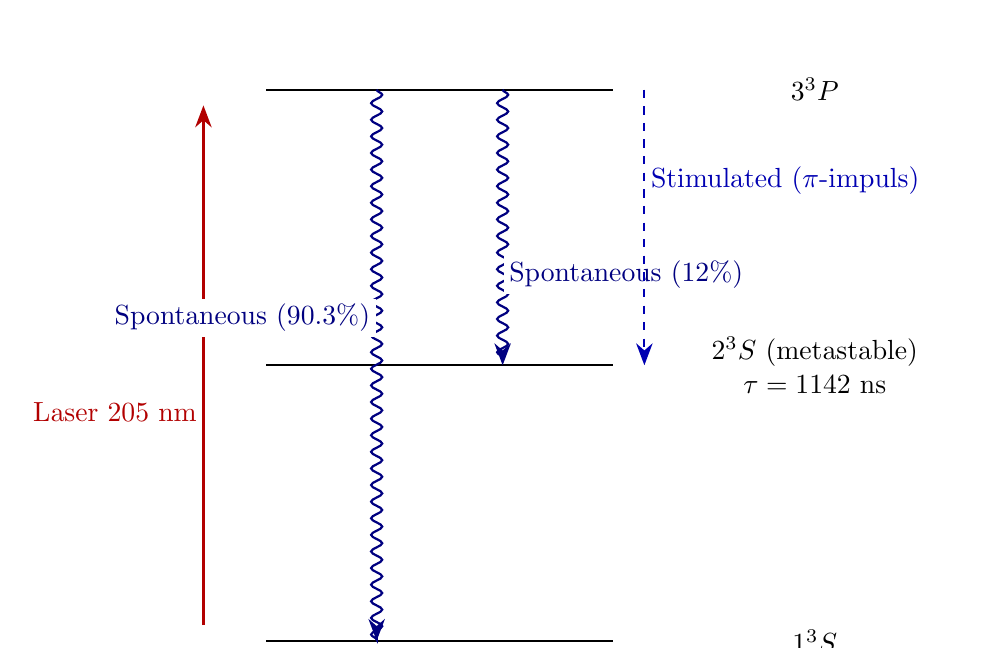
\begin{tikzpicture}[
  level/.style={draw, thick, minimum width=3.5cm, align=center},
  >={Stealth[scale=1.2]},
  pump/.style={->, thick, red!70!black},
  stim/.style={->, thick, blue!70!black, dashed},
  spon/.style={->, thick, decorate, decoration={snake, amplitude=2pt, segment length=6pt}, blue!50!black}
]

% --- Położenie poziomów energetycznych (oś Y) ---
\coordinate (G) at (0,0);   % Stan podstawowy
\coordinate (M) at (0,3.5); % Stan metastabilny
\coordinate (E) at (0,7);   % Stan wzbudzony

% --- Rysowanie poziomów ---
\draw[level] (-2.2,0) -- (2.2,0) node[right, xshift=0.8cm] {\(1^3S\)};
\draw[level] (-2.2,3.5) -- (2.2,3.5) node[right, xshift=0.8cm] {\(2^3S\) (metastable) \\ \(\tau = 1142\) ns};
\draw[level] (-2.2,7) -- (2.2,7) node[right, xshift=0.8cm] {\(3^3P\)};

% --- 1. Wzbudzenie laserowe (główna strzałka pompy) ---
\draw[pump] (-3,0.2) -- (-3,6.8) 
    node[midway, left, yshift=-0.6cm, fill=white, inner sep=2pt] {Laser 205 nm};

% --- 2. Rozpad spontaniczny z powrotem do stanu podstawowego (dominujący) ---
\draw[spon] (-0.8,7) -- (-0.8,0) 
    node[midway, left, yshift=0.6cm, fill=white, inner sep=2pt] {Spontaneous (90.3\%)};

% --- 3. Rozpad spontaniczny do stanu 2^3S (pożądany kanał) ---
\draw[spon] (0.8,7) -- (0.8,3.5) 
    node[midway, right, yshift=-0.6cm, fill=white, inner sep=2pt] {Spontaneous (12\%)};

% --- 4. Rozpad wymuszony (stymulowany) do 2^3S - metoda zwiększająca wydajność ---
\draw[stim] (2.6,7) -- (2.6,3.5) 
    node[midway, right, yshift=0.6cm, fill=white, inner sep=2pt] {Stimulated (\(\pi\)-impuls)};

% --- Opis procesu pod schematem ---
% \node at (0, -1.8) { \textbf{Schemat kaskady:} \(1^3S \xrightarrow{205\text{ nm}} 3^3P \xrightarrow{12\%} 2^3S\) };

% --- Dodatknotka o wydajności ---
% \node at (0, -2.8) [text width=10cm, align=center, font=\small] {
    % Uwaga: Stosując technikę STIRAP lub szybkie wygaszanie pola laserowego, 
    % można zwiększyć populację stanu \(2^3S\) kosztem rozpadu do \(1^3S\).
% };

\end{tikzpicture}
% \end{document}}
% \missingfigure{Jablonski diagram of o-Ps excitation}
\caption[Metastable positronium: Jabłoński diagram]{Jabłoński diagram of metastable $2^3S$ o-Ps state generation.}
\label{fig:jab}
\end{figure}

It is possible to create even longer-lived states, such as Rydberg states (with mean lifetimes in the range of milliseconds), but such states are more susceptible to electric field gradients  due to their large electric polarisability \(\alpha\) ($\alpha\propto n^6$, where \(n\) is the principal quantum number)~\cite{Cassidy_2018,Mariazzi_Caravita_Doser_Nebbia_Brusa_2020}.

\section[Production of a metastable 23S positronium beam]{Production of a metastable $2^3S$ positronium beam}

In order to measure the gravitational effect on positronium, one must first obtain a beam of metastable positronium atoms. Such a beam can be obtained in a two-step process: converting positrons ($e^+$) into a positronium cloud, and then selecting positronium atoms with the selected velocities and exciting them as shown in figure \ref{fig:jab}.

Throughout this thesis, the $x$-axis is aligned with the mean propagation direction of the positronium beam. The $y$-axis is vertical and defines the sensitive direction, along which gravitational effects are measured through a displacement of the fringe pattern. The $z$-axis completes a right-handed coordinate system. The gratings are periodic along the $y$-direction, with their bars aligned along the $z$-direction.

Positrons are produced via \(\beta^+\) decay of a $^{22}$Na source, and then are slowed down to energies of a few eV using a neon moderator and a Surko trap. Then they are implanted into a silicon converter containing nanochannels with diameters of 7--10 nm, where they diffuse into the SiO$_2$ walls, combine with electrons and are emitted as Ps atoms into the surrounding vacuum~\cite{PhysRevB.81.235418}.

While positronium ions can be accelerated using techniques like electron photodetachment~\cite{Michishio_Tachibana_Suzuki_Wada_Yagishita_Hyodo_Nagashima_2012}, the lowest kinetic energy achieved so far for a positronium beam has been 1 eV~\cite{Fayer_2015}; however, to perform experiments on gravitational interaction, one should ideally obtain a kinetic energy of the atoms of around 50 meV (which will be shown later), which is of the order of room-temperature energies. To obtain such a beam, one can use Doppler selection to choose and excite only positronium atoms with a selected velocity component along the horizontal $x$ axis, and then collimate them using a single slit (particularly because the experimental geometry is two-dimensional, so the beam can be divergent along the orthogonal horizontal $z$ axis). 
This method was shown in~\cite{PhysRevA.99.033405}: after creating a bunch of positronium atoms in vacuum, orthopositronium atoms are excited by a nanosecond ultraviolet laser pulse of a wavelength $\lambda=205$ nm perpendicular to the propagation direction from the $1^3S$ state to the $3^3P$ state. 
% The laser wavelength is Doppler-shifted, so that only positronium atoms with the matching velocity are resonantly excited and survive (within the tolerance determined by the laser spectral bandwidth and the Doppler profile), and atoms that are not excited decay quickly. 
The laser frequency is tuned so that, due to the Doppler effect, only positronium atoms with a specific matching velocity are resonantly excited and survive.
By choosing the delay between production and excitation, one can select the velocity of the resulting beam with a precision (velocity spread) of $10^4$ \si{\metre\per\second}. 
% The state $3^3P$ de-excites to $2^3S$ with a branching ratio $\sim9.7\%$.
A diagram of this method is shown in Figure \ref{fig:doppler}.

\begin{figure}[ht!]
    \centering
    \resizebox{0.75\textwidth}{!}{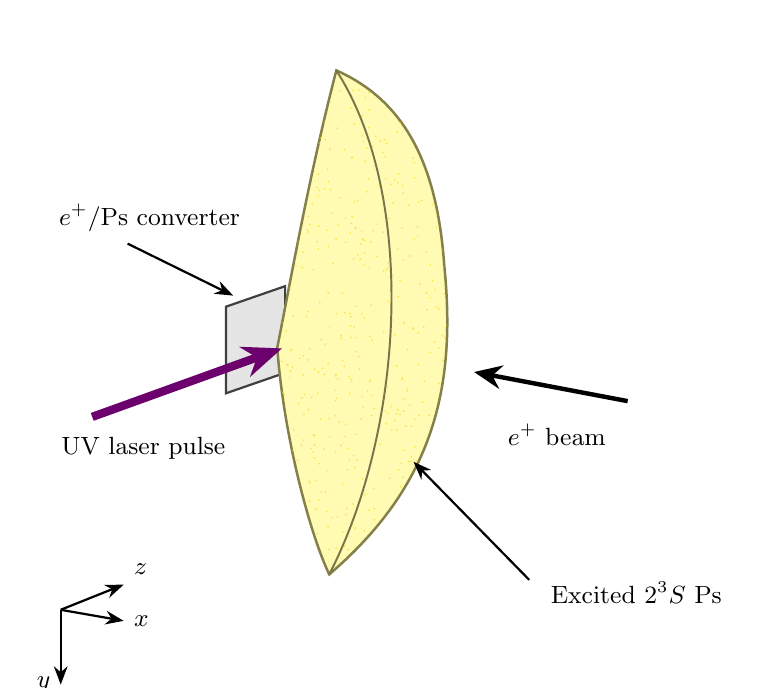
\begin{tikzpicture}[
    x=1cm,y=1cm,>=Stealth,font=\small,
    annotation/.style={->,line width=0.8pt},
    outline/.style={draw=black!75,line width=0.8pt}
]
% Converter, seen in perspective.
\filldraw[outline,fill=gray!20]
    (2.65,2.65) -- (3.40,2.91) -- (3.40,4.01) -- (2.65,3.75) -- cycle;
% Sheet of excited positronium, shown in perspective.
\path[fill=yellow!30,draw=yellow!45!black,line width=0.9pt]
    (4.05,6.75)
    .. controls (3.70,5.40) and (3.47,4.08) .. (3.30,3.23)
    .. controls (3.38,2.10) and (3.72,0.85) .. (3.96,0.35)
    .. controls (5.28,1.48) and (5.58,2.72) .. (5.42,4.28)
    .. controls (5.33,5.57) and (4.91,6.37) .. (4.05,6.75) -- cycle;
\begin{scope}
    \clip (4.05,6.75)
        .. controls (3.70,5.40) and (3.47,4.08) .. (3.30,3.23)
        .. controls (3.38,2.10) and (3.72,0.85) .. (3.96,0.35)
        .. controls (5.28,1.48) and (5.58,2.72) .. (5.42,4.28)
        .. controls (5.33,5.57) and (4.91,6.37) .. (4.05,6.75) -- cycle;
    \pgfmathsetseed{1741}
    \foreach \i in {1,...,550}{
        \pgfmathsetmacro{\px}{3.25+2.35*rnd}
        \pgfmathsetmacro{\py}{0.35+6.4*rnd}
        \fill[yellow!70!orange,opacity=0.6] (\px,\py) circle[radius=0.012];
    }
\end{scope}
\draw[yellow!40!black,line width=0.7pt]
    (4.05,6.75) .. controls (5.08,5.15) and (4.91,2.19) .. (3.96,0.35);
% Incident beams.
\draw[-{Stealth[length=5mm,width=4mm]},violet!85!black,line width=3pt]
    (0.95,2.35) -- (3.36,3.22);
\node[below,align=center] at (1.60,2.22) {UV laser pulse};
\draw[-{Stealth[length=3.5mm,width=3mm]},black,line width=1.6pt]
    (7.75,2.55) -- (5.80,2.92);
\node[below] at (6.85,2.38) {$e^+$ beam};
% Component labels.
\node[anchor=east] at (2.95,4.88) {$e^+$/Ps converter};
\draw[annotation] (1.40,4.55) -- (2.74,3.89);
\node[anchor=west] at (6.65,0.12) {Excited $2^3S$ Ps};
\draw[annotation] (6.50,0.28) -- (5.03,1.78);
% Coordinate triad, matching the reference image.
\begin{scope}[xshift=-2cm,yshift=-0.5cm]
\draw[annotation] (2.55,0.40) -- (3.35,0.26) node[right] {$x$};
\draw[annotation] (2.55,0.40) -- (2.55,-0.55) node[left] {$y$};
\draw[annotation] (2.55,0.40) -- (3.35,0.72) node[above right] {$z$};
\end{scope}
\end{tikzpicture}}
    \caption[Positronium production and Doppler selection]{Schematic of positronium production and Doppler selection, showing the incident positron beam, the $e^+$/Ps converter, the UV laser pulse, and the excited $2^3S$ positronium. Adapted from Mariazzi \emph{et~al.}~\cite{Mariazzi_Caravita_Doser_Nebbia_Brusa_2020}}
    \label{fig:doppler}
\end{figure}

Table \ref{tab:efficiency} lists the efficiencies of the particular steps of this method based on current knowledge.
% \todo{describe creation method}

\begin{table}[ht!]
    \centering
    \begin{tabular}{@{}lc@{}}
    \toprule
    Process & Efficiency \\
    \midrule
    $e^+\to$ Ps conversion (in room temperature energies) &  28\%\todo{are these values correct?} ~\cite{Mariazzi_Caravita_Zimmer_Rienacker_Camper_Belov_Bonomi_Brusa_Castelli_Consolati_etal._2021}\\
    $1^3S\to3^3P$ conversion & 
    % $\sim$0.15\cite{PhysRevLett.132.083402} \\
    $\sim14\%$~\cite{Amsler_Antonello_Belov_Bonomi_Brusa_Caccia_Camper_Caravita_Castelli_Cerchiari_etal._2019}
    \\
    $3^3P\to2^3S$ stimulated conversion & 
    % $\sim$0.15\cite{PhysRevLett.132.083402} \\
    $\sim30\%$~\cite{Antonello_Belov_Bonomi_Brusa_Caccia_Camper_Caravita_Castelli_Cerchiari_Comparat_etal._2019}
    \\
    overall & $\sim1.18\%$ \\
    \bottomrule
    \end{tabular}
    \caption[Efficiencies of metastable positronium production steps]{Efficiency of $e^+\to2^3S$ positronium conversion steps as of 2026. Assuming a bunch of $10^7$ positrons, we can obtain $1.2\times10^5$ $2^3S$ positronium atoms per bunch.}
    \label{tab:efficiency}
\end{table}

Recent studies indicate that this method can yield up to $10^5$ Ps atoms at a given horizontal velocity $v_h$; after collimation, this gives a flux of  $N_a=123\,\theta_{mrad}$, where $\theta_{mrad}$ is the angle of divergence in milliradians. 

\section{Multiphoton detector for the detection of positronium annihilation}

\noindent Positronium is a short-lived bound state and therefore cannot be observed
directly. Instead, it is identified through its annihilation products. Depending on its spin state and interaction with the surrounding medium, positronium annihilation results predominantly in two or three photons, whose total energy is approximately \(2m_ec^2=1022\)~keV. Positronium atoms can be used as an excellent probe for both fundamental physics and medical physics applications.  In recent years, the J-PET Collaboration has demonstrated that the J-PET system can be used for studies of positronium properties and decays, including positronium imaging and tests of discrete symmetries~\cite{doi:10.1126/sciadv.abh4394,moskal2021testing,moskal2024discrete,Moskal2019,moskal2024positronium}.

A PET scanner consists of rings of detection elements around the region of interest.A conventional PET scanner detects two approximately back-to-back 511~keV annihilation photons in temporal coincidence. The positions of their interactions define a line of response (LOR) along which the annihilation occurred. By combining all coincidence events of a PET scanner, the spatial distribution of positron annihilations can be calculated in three dimensions.
%
\begin{figure}[ht!]
    \centering
    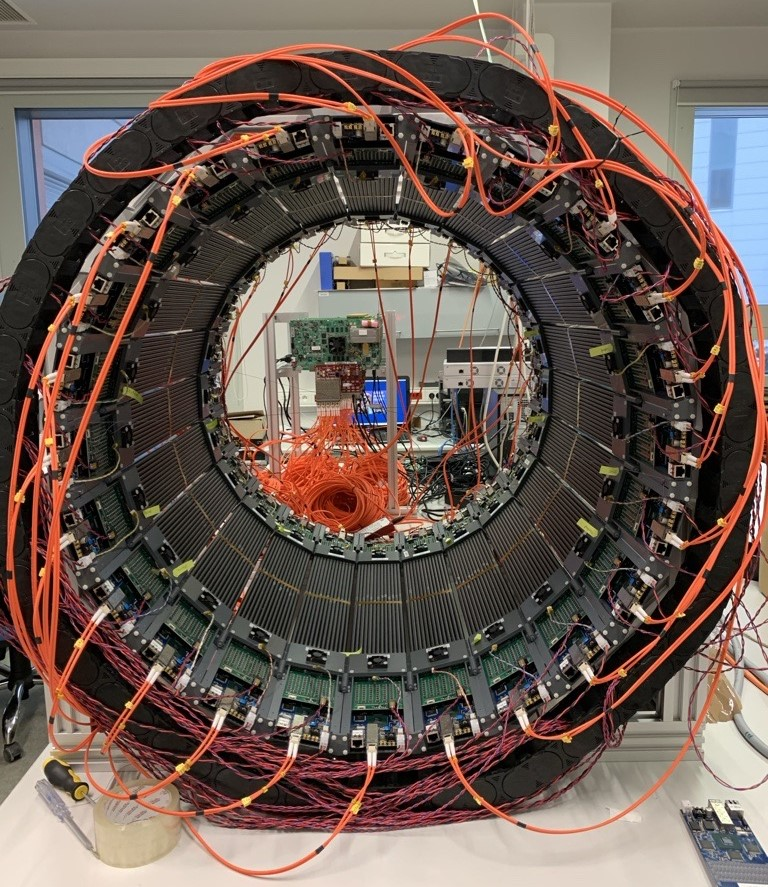
\includegraphics[width=0.5\linewidth]{modularjpet.jpg}
    \caption[Modular J-PET detector in the laboratory]{Photograph of the Modular J-PET detector in the laboratory. It consists of 24 standalone detector units~\cite{moskal2024positronium}.}
    \label{fig:modularjpet}
\end{figure}

However, for the studies of positronium decays, it is of utmost importance that the detector should be able to register events with more than two photons simultaneously. This is especially important for the detection of three photons emitted in the decay of ortho-positronium as well as for the measurements in which the annihilation photons are registered together with additional prompt photons. The Jagiellonian Positron Emission Tomograph (J-PET) detector is made of long plastic scintillator strips (see Fig.\ref{fig:modularjpet}). Due to the triggerless data acquisition, it can register multiple photons simultaneously~\cite{moskal2024positronium}.
% \twemoji{sob}
%
A feasibility study has been performed with two modular J-PET detectors in a positron beamline. The obtained time-of-flight resolution was about 125~ps ($\sigma$) and the annihilation-vertex resolution along the beam direction was about 4~mm ($\sigma$)~\cite{Sharma_Povolo_Mariazzi_Korcyl_Kacprzak_Kumar_Niedźwiecki_Baran_Beyene_Brusa_etal._2024}. Importantly, the obtained values enable us to distinguish between annihilation vertices separated by 10--20~mm, which is the requirement of the grating--stopper readout studied in the present thesis.

In the positronium-beam experiments considered in this thesis, such a multiphoton detector can be used to determine where the positronium atom annihilates along the experimental apparatus. In particular, the detector must distinguish annihilations occurring in vacuum from those occurring on the material gratings or on the stopper. The reconstructed annihilation position and photon multiplicity therefore provide the information required for the third-grating detection method introduced in Sec.~\ref{sec:third}~\cite{Sharma_Povolo_Mariazzi_Korcyl_Kacprzak_Kumar_Niedźwiecki_Baran_Beyene_Brusa_etal._2024}.
Modular J-PET detection units have therefore been proposed and experimentally evaluated as position-sensitive detectors for inertial-sensing studies with positronium atoms~\cite{Sharma_Povolo_Mariazzi_Korcyl_Kacprzak_Kumar_Niedźwiecki_Baran_Beyene_Brusa_etal._2024}.

It can be easily calculated from the free fall equation of motion that the mean displacement of a positronium atom in Earth's gravitational field over its lifetime lies in the sub-nanometre range, which makes any deflection practically undetectable. 
A solution to this challenge will be introduced and discussed in section \ref{sec:third}.

\chapter{Atomic deflectometry and interferometry for gravitational measurements}

\section{Principles of atomic deflectometry and interferometry}

Atomic interferometry is an area of physics that utilises the phenomenon of wave interference (superposition of coherent waves) using matter waves. 
%Although wave-particle duality was introduced by Louis de Broglie in the 1920s, the first experimental demonstrations of atomic interference were reported in the early 1990s\cite{Cronin_Schmiedmayer_Pritchard_2009}. 
Although matter-wave interference had been demonstrated earlier, modern separated-beam atom interferometers were realized in the early 1990s, notably the three-grating sodium interferometer of Keith \emph{et~al.}~\cite{Keith1991}.
% \todo{say more about interferometry and modern physics}
Since its experimental confirmation, atomic interferometry has been widely applied in fundamental physics experiments where high sensitivity is needed, such as gravimetry~\cite{Vovrosh_Dragomir_Stray_Boddice_2023}, tests of relativistic theories (such as equivalence principle tests), measurements of fundamental constants (\(\alpha\), \(G\) and \(\hbar\)) and high-precision inertial sensing (with applications in space probes).
% 
% In this thesis, I will compare two systems: Moir\'e deflectometry and Mach--Zehnder interferometry.

The systems considered in this thesis show two distinct approaches: whereas Mach--Zehnder interferometry is based on quantum matter-waves interferometry, moir\'e deflectometry is a fully classical method based on particle trajectories.

\section{Moir\'e deflectometry}\label{sec:moire}

A moir\'e (from French: shimmering, rippled) pattern is a pattern produced by the light shadow when two or more overlaid repeating opaque patterns (e.g. grids or parallel lines) form an optical illusion of a new, larger repeating pattern. The effect arises when the two patterns are slightly rotated relative to each other, or when the spacing of one of the patterns is slightly different from that of the other, causing the lines to periodically fall in and out of alignment. An example of such a pattern is shown in Figure \ref{fig:moi3d}.

\begin{figure}[ht!]
    \centering
        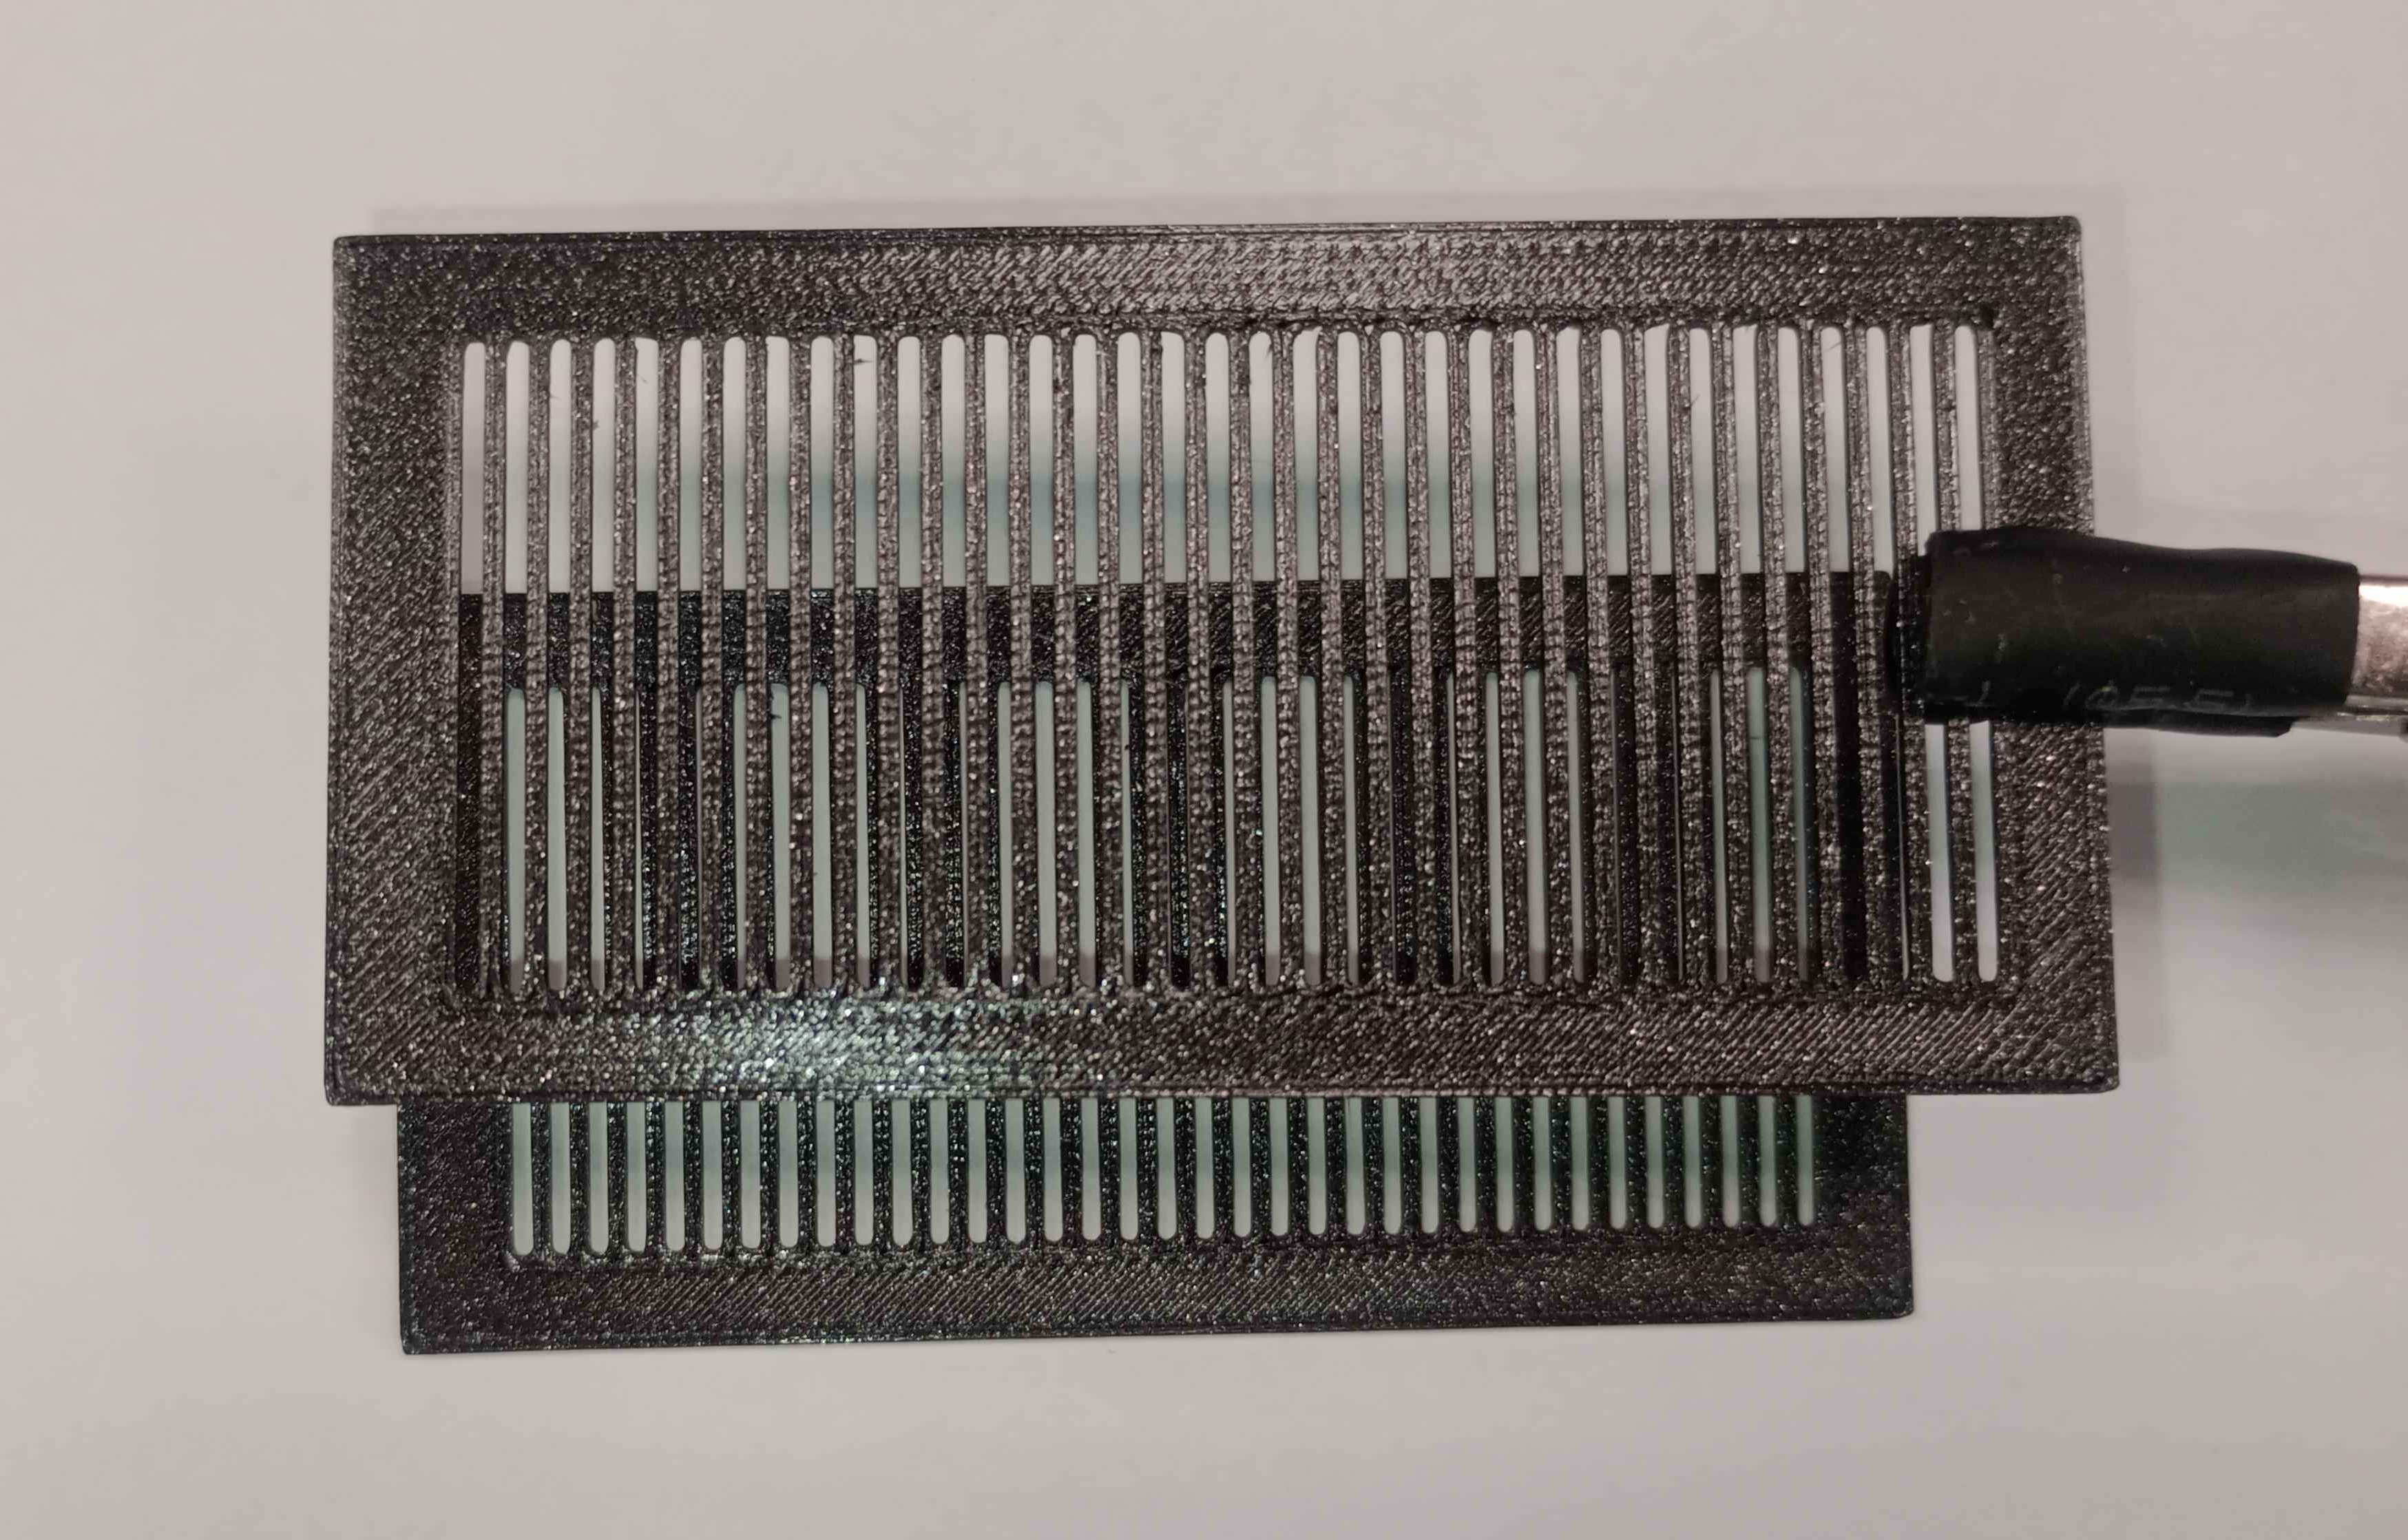
\includegraphics[width=0.8\linewidth]{moire-3d.png}
        \caption[Example of a moir\'e pattern]{A moir\'e pattern, created with 3D-printed elements. Both gratings have the same period \(d=2\) mm and opening width \(a=1\) mm.}
    \label{fig:moi3d}
\end{figure}

Such an effect can be used in high-precision experiments, due to its high sensitivity to small changes in the displacement of the patterns. 
% \todo{write a transition between pattern and deflectometry}
The effect can also be observed with particles instead of light: in this case, with stationary gratings, the position of the moir\'e pattern is affected by a change in the path of motion of the particles. When the particles pass through the first grating, they create a periodic intensity distribution, which then falls on the second grating.  The displacement of the distribution relative to the second grating produces a displacement of the moir\'e pattern. The measurement of this displacement allows determining the deflection angle of the trajectories, and hence the acting force.

In fundamental physics, moir\'e patterns are employed in deflectometers: highly sensitive instruments used to measure small forces that curve the particles' trajectories. A typical deflectometer consists of a collimated particle beam, a pair of gratings with an equal grating period \(d\) and an equal grating width \(a\) (hence the same open fraction \(f=a/d\)), and a screen. (Alternatively, a setup with three gratings can be used; in this configuration, the first grating acts as a source of spatial coherence, so the original beam does not need to be collimated.) The distances between the particle source and the first grating, between the gratings, and between the second grating and the screen are equal and denoted by \(L\).
The particle beam, while passing through the gratings, is blocked when it meets the opaque regions of the gratings, and the transmitted part of the beam produces a moir\'e pattern with a period \(d\) on the screen. 
The resulting pattern can be compared with a reference pattern of light passing through the same gratings (since light is not deflected by the force on a laboratory scale), and the relative shift between the two patterns yields the deflection. Alternatively, one can reverse the direction of the force (e.g. by rotating the apparatus by 180\si\degree) to observe a pattern shifted in the opposite direction, but of the same magnitude. This principle is illustrated in Figure \ref{fig:moired}.

\begin{figure}[ht!]
    \centering
    \resizebox{0.95\textwidth}{!}{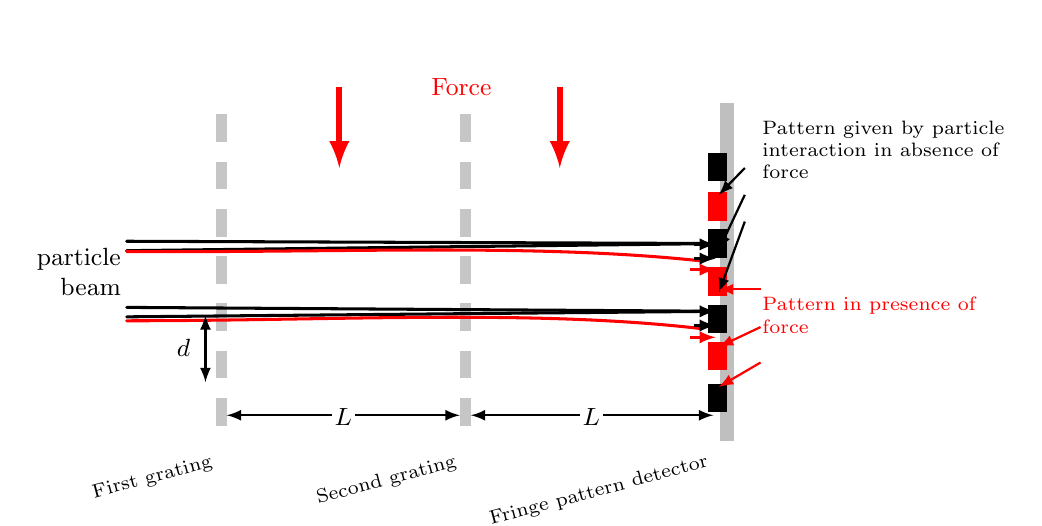
\begin{tikzpicture}[
  x=1cm,y=1cm,
  beam/.style={line width=1.1pt,line cap=round},
  force/.style={-latex,red,line width=2.3pt},
  label/.style={font=\small},
  smalllabel/.style={font=\scriptsize},
  dim/.style={latex-latex,line width=0.8pt},
  callout/.style={-latex,line width=0.8pt},
  redcallout/.style={-latex,red,line width=0.8pt}
]
  \def\gOne{1.25}
  \def\gTwo{4.35}
  \def\det{7.55}

  \foreach \x in {\gOne,\gTwo}{
    \foreach \y in {0.45,1.05,1.65,2.25,2.85,3.45,4.05}{
      \draw[gray!45,line width=4pt] (\x,\y) -- (\x,\y+0.35);
    }
  }

  \draw[gray!50,line width=5pt] (\det+0.12,0.25) -- (\det+0.12,4.55);
  \foreach \y/\c in {0.62/black,1.15/red,1.62/black,2.10/red,2.58/black,3.05/red,3.55/black}{
    \draw[\c,line width=7pt] (\det,\y) -- (\det,\y+0.36);
  }

  \node[label,align=right,anchor=east] at (0.10,2.40) {particle\\beam};
  \node[label,red] at (4.30,4.75) {Force};
  \draw[force] (2.75,4.75) -- (2.75,3.72);
  \draw[force] (5.55,4.75) -- (5.55,3.72);

  \foreach \dy in {-0.05,0.07}{
    \draw[beam,black] (0.05,2.72+\dy) -- (\det-0.20,2.76+0.03*\dy);
    \draw[beam,black] (0.05,1.88+\dy) -- (\det-0.20,1.90+0.03*\dy);
  }
  \draw[beam,red] (0.05,2.66) .. controls (2.7,2.64) and (5.2,2.77) .. (\det-0.20,2.54);
  \draw[beam,red] (0.05,1.78) .. controls (2.7,1.78) and (5.2,1.93) .. (\det-0.20,1.68);

  \foreach \y in {2.57,2.75,1.72,1.90}{
    \draw[-latex,line width=1pt] (\det-0.30,\y) -- (\det-0.02,\y);
  }
  \draw[-latex,red,line width=1pt] (\det-0.34,2.43) -- (\det-0.02,2.43);
  \draw[-latex,red,line width=1pt] (\det-0.34,1.57) -- (\det-0.02,1.57);

  \draw[dim] (\gOne-0.20,1.00) -- (\gOne-0.20,1.85);
  \node[label,fill=white,inner sep=1pt] at (\gOne-0.48,1.43) {$d$};

  \draw[dim] (\gOne+0.07,0.58) -- (\gTwo-0.07,0.58);
  \node[label,fill=white,inner sep=1pt] at ({(\gOne+\gTwo)/2},0.56) {$L$};
  \draw[dim] (\gTwo+0.07,0.58) -- (\det-0.05,0.58);
  \node[label,fill=white,inner sep=1pt] at ({(\gTwo+\det)/2},0.56) {$L$};

  \node[smalllabel,align=center,rotate=15,anchor=east] at (\gOne,0.02) {First grating};
  \node[smalllabel,align=center,rotate=15,anchor=east] at (\gTwo,0.02) {Second grating};
  \node[smalllabel,align=center,rotate=15,anchor=east] at (\det,0.02) {Fringe pattern detector};

  \node[smalllabel,align=left,anchor=west] (absent) at (8.00,3.95) {Pattern given by particle\\interaction in absence of\\force};
  \draw[callout] (7.90,3.72) -- (\det+0.02,3.38);
  \draw[callout] (7.90,3.38) -- (\det+0.02,2.68);
  \draw[callout] (7.90,3.04) -- (\det+0.02,2.14);

  \node[smalllabel,align=left,anchor=west,red] at (8.00,1.85) {Pattern in presence of\\force};
  \draw[redcallout] (8.10,2.18) -- (\det+0.02,2.18);
  \draw[redcallout] (8.10,1.70) -- (\det+0.02,1.45);
  \draw[redcallout] (8.10,1.25) -- (\det+0.02,0.94);
\end{tikzpicture}}
    \caption[Operating principle of the moir\'e deflectometer]{The principle of operation of a two-grating moir\'e deflectometer. In the absence of a force, particles form a black pattern on a screen; in the presence of a force, they form a downward-shifted red image. The vertical and horizontal axes are not shown to scale. Adapted from Mariazzi \emph{et~al.}~\cite{Mariazzi_Caravita_Doser_Nebbia_Brusa_2020}.}
    \label{fig:moired}
    
\end{figure}

A moir\'e deflectometer was proposed by the AEgIS collaboration to test the gravitational interaction of antiprotons, and experiments were conducted in 2014~\cite{Aghion2014}. In a proof-of-concept experiment conducted at CERN's Antiproton Decelerator, a moir\'e pattern was obtained and a microscopic relative shift between the antiproton moir\'e pattern and the Talbot--Lau light pattern was observed. A moir\'e deflectometer experiment for antihydrogen is under preparation by the AEgIS collaboration as of 2025~\cite{Ferguson_AEḡISCollaboration_2025}.

\section{Mach--Zehnder interferometry}\label{sec:mach}

A Mach--Zehnder interferometer is an optical device used to measure the relative phase difference between two light beams.
The device was originally created by Ludwig Zehnder in 1891 and refined by Ludwig Mach in 1892~\cite{LudwigMach_1892}.
%, it took physicists over 100 years to construct a matter wave Mach--Zehnder interferometer -- an electronic (i.e. using electrons) interferometer in 2003\cite{Ji_Chung_Sprinzak_Heiblum_Mahalu_Shtrikman_2003}.
The Mach--Zehnder geometry was later extended from optical to matter waves, first in atom interferometers based on diffraction gratings and subsequently in electronic interferometers in mesoscopic systems~\cite{Cronin_Schmiedmayer_Pritchard_2009,Ji_Chung_Sprinzak_Heiblum_Mahalu_Shtrikman_2003}.

The idea behind the interferometer is to divide the original beam by a beam splitter into two beams: the test beam and the reference beam, each beam is then reflected by a mirror and both beams are recombined in the second beam splitter, as shown in Figure \ref{fig:mach-optical}.%\todo{maybe insert an image of a 'classical' interferometer here?} 
To construct such an interferometer using matter waves, one can replace optical beam splitters with diffraction gratings, laser beams (via Raman or Bragg transitions) or magnetic mirrors.

\begin{figure}[ht!]
\centering
\resizebox{0.7\textwidth}{!}{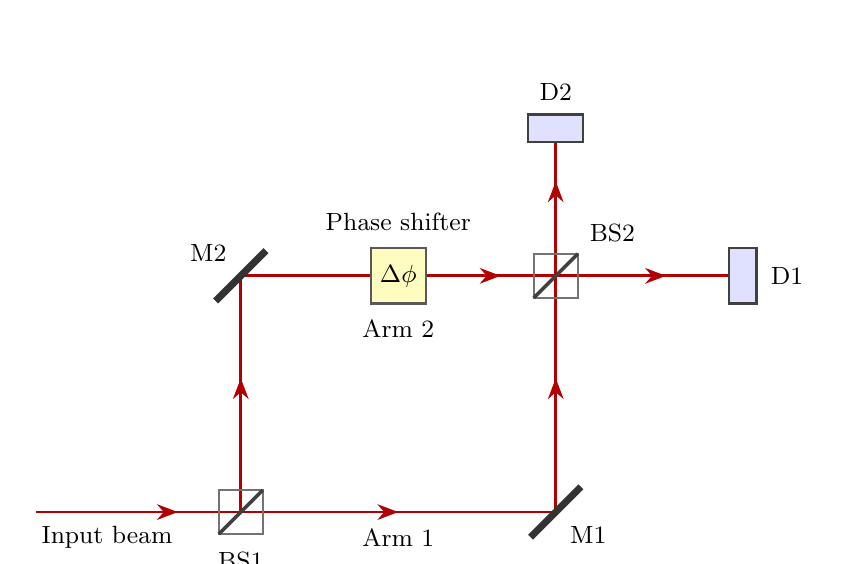
\begin{tikzpicture}[
    x=1cm,y=1cm,
    >=Stealth,
    font=\small,
    beam/.style={draw=red!70!black,line width=1pt},
    beamsplitter/.style={draw=black!75,line width=1.3pt},
    mirror/.style={draw=black!80,line width=2.5pt},
    detector/.style={fill=blue!12,draw=black!75,line width=0.8pt},
    phaseshifter/.style={fill=yellow!25,draw=black!65,line width=0.8pt}
]
% Optical components.
\coordinate (BS1) at (0,0);
\coordinate (M1) at (4,0);
\coordinate (M2) at (0,3);
\coordinate (BS2) at (4,3);

% Beam paths; arrows are placed away from the optical components.
\draw[beam] (-2.6,0) -- (M1) -- (BS2);
\draw[beam] (BS1) -- (M2) -- (6.2,3);
\draw[beam] (BS2) -- (4,4.7);
\draw[beam,->] (-2.3,0) -- (-0.8,0);
\draw[beam,->] (1.2,0) -- (2,0);
\draw[beam,->] (4,0.9) -- (4,1.7);
\draw[beam,->] (0,0.9) -- (0,1.7);
\draw[beam,->] (2.6,3) -- (3.3,3);
\draw[beam,->] (4.7,3) -- (5.4,3);
\draw[beam,->] (4,3.6) -- (4,4.2);

% Beam-splitter cubes with their partially reflecting interfaces.
\foreach \component in {BS1,BS2}{
    \draw[draw=black!55,line width=0.7pt]
        (\component) ++(-0.28,-0.28) rectangle ++(0.56,0.56);
    \draw[beamsplitter]
        (\component) ++(-0.28,-0.28) -- ++(0.56,0.56);
}
\node[below,inner sep=3pt] at (0,-0.4) {BS1};
\node[above right,inner sep=5pt] at (4.25,3.25) {BS2};

% Both mirrors are oriented at 45 degrees to the incident beams.
\foreach \component in {M1,M2}{
    \draw[mirror] (\component) ++(-0.32,-0.32) -- ++(0.64,0.64);
}
\node[below right,inner sep=5pt] at (M1) {M1};
\node[above left,inner sep=5pt] at (M2) {M2};

% Output detectors.
\draw[detector] (6.2,2.65) rectangle (6.55,3.35);
\node[right,inner sep=5pt] at (6.55,3) {D1};
\draw[detector] (3.65,4.7) rectangle (4.35,5.05);
\node[above,inner sep=5pt] at (4,5.05) {D2};

% Phase shifter in the upper arm.
\draw[phaseshifter] (1.65,2.65) rectangle (2.35,3.35);
\node at (2,3) {$\Delta\phi$};
\node[above,align=center] at (2,3.45) {Phase shifter};

% Labels are offset from the light paths.
\node[below,inner sep=5pt] at (-1.7,0) {Input beam};
\node[below,inner sep=6pt] at (2,0) {Arm 1};
\node[below,inner sep=6pt] at (2,2.65) {Arm 2};
\end{tikzpicture}}
\caption[Optical Mach--Zehnder interferometer]{Schematic of an optical Mach--Zehnder interferometer. The input beam is divided at beam splitter BS1, reflected by mirrors M1 and M2, and recombined at beam splitter BS2. A phase shifter introduces a relative phase shift \(\Delta\phi\) between the arms; detectors D1 and D2 record the two output beams.}
\label{fig:mach-optical}
\end{figure}

The scheme of the Mach--Zehnder interferometer in the context of positronium gravity measurements is shown in Figure \ref{fig:machidea}. Its main benefit in comparison with the moir\'e deflectometer is the possibility of using laser standing waves as gratings, which offers two advantages: no particles are lost by annihilation in the gratings, and the grating period can be reduced by about two orders of magnitude. 

A standing light wave with wave vector $k$ produces a spatially periodic intensity, $I(y)\propto\cos^{2}(ky)$, and hence a periodic optical-dipole potential acting on the atom; this potential is what plays the role of a diffraction grating. By tuning the depth and the interaction time of the potential, the fraction of atoms transferred between the coupled momentum states can be controlled, so that the standing wave acts as a coherent beam splitter or mirror for the matter wave~\cite{Oberthaler_2002,Dürr_Rempe_1999}.

\begin{figure}[ht!]
    \centering
    % \missingfigure{scheme of Mach--Zehnder interferometer from poster}
    % \includegraphics[width=0.8\textwidth]{}
    \resizebox{0.8\textwidth}{!}{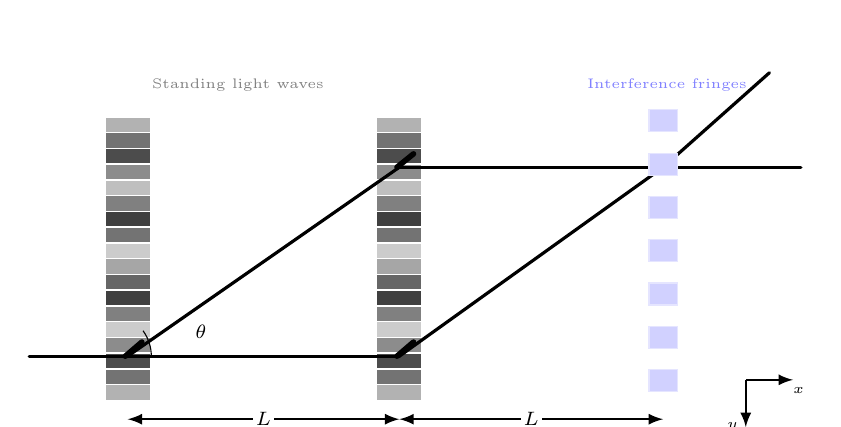
\begin{tikzpicture}[
  x=1cm,y=1cm,
  ray/.style={line width=1.15pt,line cap=round},
  dim/.style={latex-latex,line width=0.8pt},
  label/.style={font=\scriptsize},
  smalllabel/.style={font=\tiny},
  fringe/.style={fill=blue!18,draw=blue!10}
]
  \def\gA{1.30}
  \def\gB{4.75}
  \def\scr{8.10}

  % \node[smalllabel,font=\scriptsize\bfseries] at (4.60,5.85) {Mach--Zehnder interferometer};
  \node[smalllabel,black!50] at (2.70,4.90) {Standing light waves};
  \node[smalllabel,blue!50] at (8.15,4.90) {Interference fringes};

  \foreach \x in {\gA,\gB}{
    \foreach \y/\shade in {0.90/30,1.10/55,1.30/70,1.50/45,1.70/20,1.90/50,2.10/75,2.30/60,2.50/35,2.70/20,2.90/55,3.10/75,3.30/50,3.50/25,3.70/45,3.90/70,4.10/55,4.30/30}{
      \fill[black!\shade] (\x-0.28,\y) rectangle (\x+0.28,\y+0.18);
    }
  }

  \draw[ray] (0.05,1.45) -- (\gA,1.45);
  \draw[ray] (\gA,1.45) -- (\gB,3.85);
  \draw[ray] (\gB,3.85) -- (\scr,3.85);
  \draw[ray] (\gA,1.45) -- (\gB,1.45);
  \draw[ray] (\gB,1.45) -- (\scr,3.85);
  \draw[ray] (\scr,3.85) -- (9.85,3.85);
  \draw[ray] (\scr,3.85) -- (9.45,5.05);

  \draw[ray,line width=2pt] (\gA-0.03,1.45) -- (\gA+0.18,1.63);
  \draw[ray,line width=2pt] (\gB-0.03,1.45) -- (\gB+0.18,1.63);
  \draw[ray,line width=2pt] (\gB-0.03,3.85) -- (\gB+0.18,4.02);

  \draw[thin] (\gA+0.30,1.45) arc[start angle=0,end angle=36,radius=0.55];
  \node[label] at (\gA+0.93,1.76) {$\theta$};

  \foreach \y in {1.00,1.55,2.10,2.65,3.20,3.75,4.30}{
    \path[fringe] (\scr-0.18,\y) rectangle (\scr+0.18,\y+0.28);
  }

  \draw[dim] (\gA,0.65) -- (\gB,0.65);
  \node[label,fill=white,inner sep=1pt] at ({(\gA+\gB)/2},0.65) {$L$};
  \draw[dim] (\gB,0.65) -- (\scr,0.65);
  \node[label,fill=white,inner sep=1pt] at ({(\gB+\scr)/2},0.65) {$L$};

  \draw[-latex,line width=0.8pt] (9.15,1.15) -- (9.75,1.15);
  \draw[-latex,line width=0.8pt] (9.15,1.15) -- (9.15,0.55);
  \node[smalllabel] at (9.82,1.02) {$x$};
  \node[smalllabel] at (8.98,0.55) {$y$};
\end{tikzpicture}}
    \caption[Mach--Zehnder interferometer layout]{Scheme of a positronium atom beam Mach--Zehnder interferometer, in a configuration with two standing-wave light gratings and an interference fringe screen/detector. Adapted from Mariazzi \emph{et~al.}~\cite{Mariazzi_Caravita_Doser_Nebbia_Brusa_2020}.}
    \label{fig:machidea}
    
\end{figure}

Instead of using a physical grating to deflect a positronium atoms beam~\cite{Oberthaler_Bernet_Rasel_Schmiedmayer_Zeilinger_1996}, the beam is diffracted by a standing laser wave acting as an optical grating, which is known as the Kapitza-Dirac effect~\cite{Kapitza_Dirac_1933}.
In this effect, an atom passing through the grating experiences a momentum difference of \(\Delta p=2n\hbar k\), where \(n\) is a natural number.
The laser beam has to be wide enough, i. e. wider than the Talbot length \(L_T=\frac{2d^2}{\lambda_{dB}} \) (where \(d\) is the grating period, and \(\lambda_{dB}=h/mv\) is de Broglie wavelength of the particle), for the effect to operate in the Bragg regime, so the grating produces only one diffraction peak and leaves the original beam~\cite{Oberthaler_2002} (i.e. two possible momentum states \(n=0\) and \(n=1\) are possible).
The wavefunction of an atom becomes a coherent superposition of two momentum states:
\begin{equation} \lvert \psi \rangle = \frac{1}{\sqrt{2}} \left( |p \rangle + e^{\mathrm{i}\phi} |p + 2\hbar k \rangle \right).\end{equation} 
% By adjusting the interaction time and the light intensity, one can control the fraction of diffracted atoms and use the grating as a beam splitter.
Since the two beams have different momenta, they propagate in different directions, thus creating two arms of the interferometer.
% \todo{describe physical process of beam splitting (Bragg diffraction)}

In this scheme, as in most quantum Mach--Zehnder interferometers, the optical phase is replaced by the quantum phase evolution of the particle beam. In this case, the phase change does not arise from any physical obstruction on the way of the beam, but from a change of potential, which accumulates over time as a change of action \(S\), thereby changing the phase \(\phi\):
\begin{equation} 
    \phi(t)
    = \frac{S(t)}{\hbar}
    = \frac{1}{\hbar} \int_{0}^{t} \left[E_k(t')-E_p(t')\right]\,\mathrm{d}t'.
\end{equation}

For a uniform acceleration \(a\) along the sensitive direction, the phase shift can be derived in a freely falling frame. Let \(t=L/v\) be the flight time between successive grating planes, so that the total time from the first grating to the detector plane is \(2t\). In this frame, the apparatus accelerates at \(-a\), giving the following acceleration-induced displacements at times \(0\), \(t\), and \(2t\):
\begin{equation}
    \delta y_1=0,\qquad
    \delta y_2=-\frac{1}{2}at^2,\qquad
    \delta y_3=-\frac{1}{2}a(2t)^2=-2at^2.
\end{equation}
The fringe phase depends on the combination \(\delta y_1-2\delta y_2+\delta y_3\); the factor of two arises from the opposite diffraction of the two paths at the second grating~\cite{Cronin_Schmiedmayer_Pritchard_2009}. Choosing the phase convention in which positive \(a\) gives positive \(\Delta\phi\), we obtain
\begin{equation}
    \begin{aligned}
        \Delta\phi &=-\frac{2\pi}{d}
        \left(\delta y_1-2\delta y_2+\delta y_3\right)
        =-\frac{2\pi}{d}\left(at^2-2at^2\right) \\
        &=\frac{2\pi at^2}{d}.
    \end{aligned}
    \label{eq:mz-acceleration-phase}
\end{equation}


The resulting fringe pattern seen on the screen in this scenario is a sinusoidal pattern, with a period equal to the grating period; since the grating is formed by a standing wave, this period is $\lambda/2$.

In a Mach--Zehnder interferometer (and any other interferometer), to obtain clear and distinct interference fringes, the input beam has to be coherent, which is a disadvantage of this method. In a real experiment, the beam of positronium atoms must be collimated in both velocity and angle of incidence, which limits the number of atoms that can be used in the experiment.

\section{Third-grating detection scheme}\label{sec:third}

Despite proposals of atomic deflectometry/interferometry, direct detection of the gravitational deflection is not straightforward. The main difficulty is the short interrogation time with the gravitational field, limited by the mean positronium lifetime -- given Earth's gravitational acceleration and the mean lifetime of \(2^3S\) positronium, the resulting beam displacement does not exceed one nanometre. To overcome this limitation, a setup including a third grating and a stopper is introduced, as proposed in~\cite{Mariazzi_Caravita_Doser_Nebbia_Brusa_2020} and as shown in Figure \ref{fig:third}. By scanning the third grating along the \(y\)-axis and counting the positronium atoms reaching the stopper, a periodic transmission curve is obtained. Gravitational deflection shifts this curve relative to the reference measurement, converting the sub-nanometre beam displacement into a measurable shift of count modulation.

\begin{figure}[ht!]
    \centering
    \resizebox{0.95\textwidth}{!}{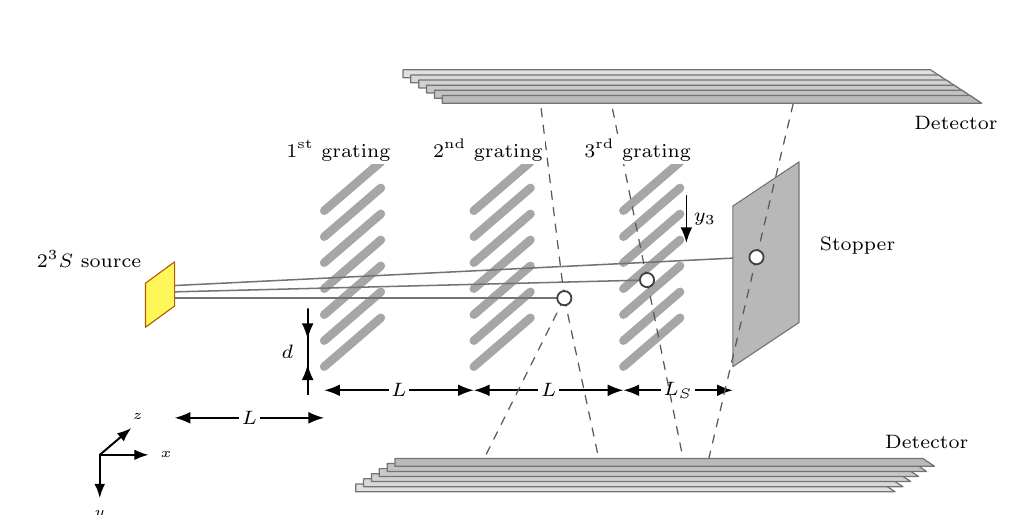
\begin{tikzpicture}[
  x=1cm,
  y=1cm,
  line cap=round,
  line join=round,
  label/.style={font=\scriptsize},
  smalllabel/.style={font=\tiny},
  beam/.style={draw=black!55,line width=0.55pt},
  photon/.style={draw=black!65,line width=0.45pt,dashed},
  dimension/.style={{Latex[length=2mm]}-{Latex[length=2mm]},line width=0.65pt},
  axis/.style={-{Latex[length=1.8mm]},line width=0.7pt}
]

  % Positronium source
  \fill[yellow!65] (-0.82,2.35) -- (-0.45,2.62) -- (-0.45,3.18)
      -- (-0.82,2.91) -- cycle;
  \draw[orange!70!black] (-0.82,2.35) -- (-0.45,2.62) -- (-0.45,3.18)
      -- (-0.82,2.91) -- cycle;
  \node[label,anchor=east] at (-0.75,3.22) {$2^3S$ source};

  % Three material gratings.  The repeated diagonal bars suggest depth.
  \foreach \gx/\name in {1.45/{1\textsuperscript{st} grating},
                          3.35/{2\textsuperscript{nd} grating},
                          5.25/{3\textsuperscript{rd} grating}} {
    \foreach \yy in {1.85,2.18,2.51,2.84,3.17,3.50,3.83} {
      \draw[black!35,line width=3.1pt]
        (\gx,\yy) -- ++(0.72,0.62);
    }
  }

  % Representative trajectories of the metastable positronium beam
  \draw[beam] (-0.45,2.72) -- (4.50,2.72);
  \draw[beam] (-0.45,2.80) -- (5.55,2.95);
  \draw[beam] (-0.45,2.88) -- (6.88,3.24);

  % Grating period d
  \draw[line width=0.65pt] (1.24,1.50) -- (1.24,2.58);
  \draw[-{Latex[length=2mm]},line width=0.65pt]
    (1.24,1.50) -- (1.24,1.88);
  \draw[-{Latex[length=2mm]},line width=0.65pt]
    (1.24,2.58) -- (1.24,2.20);
  \node[label,anchor=east] at (1.18,2.04) {$d$};

  % Equal distances between consecutive gratings
  \draw[dimension] (-0.45,1.20) -- (1.45,1.20);
  \node[label,fill=white,inner sep=1pt] at (0.50,1.20) {$L$};
  \draw[dimension] (1.45,1.55) -- (3.35,1.55);
  \node[label,fill=white,inner sep=1pt] at (2.40,1.55) {$L$};
  \draw[dimension] (3.35,1.55) -- (5.25,1.55);
  \node[label,fill=white,inner sep=1pt] at (4.30,1.55) {$L$};
  \draw[dimension] (5.25,1.55) -- (6.64,1.55);
  \node[label,fill=white,inner sep=1pt] at (5.945,1.55) {$L_S$};

  % Annihilation point and reconstructed vertical position
  % Highest beam at the stopper and middle beam at the third grating.
  \coordinate (decay) at (6.94,3.24);
  \coordinate (decaytwo) at (5.55,2.95);
  \coordinate (decaythree) at (4.50,2.72);
  \draw[-{Latex[length=2mm]},line width=0.65pt]
    (6.05,4.02) -- (6.05,3.42);
  \node[label,anchor=west] at (6.02,3.72) {$y_3$};

  % Stopper blocking the surviving positronium atoms
  \fill[black!28] (6.64,1.85) -- (7.48,2.41) -- (7.48,4.45)
      -- (6.64,3.89) -- cycle;
  \draw[black!55] (6.64,1.85) -- (7.48,2.41) -- (7.48,4.45)
      -- (6.64,3.89) -- cycle;
  \node[label,anchor=west] at (7.62,3.38) {Stopper};

  % Gamma rays from the annihilation point to opposite detector modules
  \draw[photon] (decay) -- (7.50,5.58);
  \draw[photon] (decay) -- (6.32,0.62);

  % A second reconstructed event, included as in the reference drawing
  \draw[photon] (decaytwo) -- (5.02,5.58);
  \draw[photon] (decaytwo) -- (6.02,0.62);

  % Three-photon annihilation from the third point
  \draw[photon] (decaythree) -- (4.15,5.58);
  \draw[photon] (decaythree) -- (3.45,0.62);
  \draw[photon] (decaythree) -- (4.95,0.62);

  % Annihilation points
  \draw[black!75,fill=white,line width=0.65pt] (decay) circle (0.09);
  \draw[black!75,fill=white,line width=0.65pt] (decaytwo) circle (0.09);
  \draw[black!75,fill=white,line width=0.65pt] (decaythree) circle (0.09);

  % Long scintillator modules above and below the apparatus
  \foreach \i in {0,...,5} {
    \pgfmathsetmacro{\dx}{0.10*\i}
    \pgfmathsetmacro{\dy}{0.065*\i}
    \pgfmathtruncatemacro{\detectorshade}{12+3*\i}
    \fill[black!\detectorshade]
      (2.45+\dx,5.62-\dy) -- (9.15+\dx,5.62-\dy)
      -- (9.30+\dx,5.52-\dy) -- (2.45+\dx,5.52-\dy) -- cycle;
    \draw[black!55,line width=0.45pt]
      (2.45+\dx,5.62-\dy) -- (9.15+\dx,5.62-\dy)
      -- (9.30+\dx,5.52-\dy) -- (2.45+\dx,5.52-\dy) -- cycle;
    \fill[black!\detectorshade]
      (1.85+\dx,0.36+\dy) -- (8.55+\dx,0.36+\dy)
      -- (8.70+\dx,0.26+\dy) -- (1.85+\dx,0.26+\dy) -- cycle;
    \draw[black!55,line width=0.45pt]
      (1.85+\dx,0.36+\dy) -- (8.55+\dx,0.36+\dy)
      -- (8.70+\dx,0.26+\dy) -- (1.85+\dx,0.26+\dy) -- cycle;
  }
  \node[label,anchor=west] at (8.82,4.95) {Detector};
  \node[label,anchor=west] at (8.45,0.90) {Detector};

  % Draw grating labels last so that the detector perspective does not hide them.
  \node[label,anchor=south,fill=white,inner sep=1pt] at (1.63,4.42)
    {1\textsuperscript{st} grating};
  \node[label,anchor=south,fill=white,inner sep=1pt] at (3.53,4.42)
    {2\textsuperscript{nd} grating};
  \node[label,anchor=south,fill=white,inner sep=1pt] at (5.43,4.42)
    {3\textsuperscript{rd} grating};

  % Coordinate system
  \coordinate (origin) at (-1.40,0.73);
  \draw[axis] (origin) -- ++(0.62,0);
  \draw[axis] (origin) -- ++(0,-0.55);
  \draw[axis] (origin) -- ++(0.40,0.34);
  \node[smalllabel,anchor=west] at (-0.75,0.73) {$x$};
  \node[smalllabel,anchor=north] at (-1.40,0.15) {$y$};
  \node[smalllabel,anchor=south east] at (-0.73,1.05) {$z$};

\end{tikzpicture}}
    \caption[Third-grating detection scheme]{Scheme of the third-grating detection method. Positronium atoms passing through the gratings are stopped by the stopper, while photons (dashed lines) from their annihilation (circles) are registered by the surrounding detectors. The third grating can be moved along the $y$-axis with nanometre-scale precision, as indicated by the $y_3$ arrow. The grating period and the distance between the third grating and the stopper are not shown to scale. Adapted from Mariazzi \emph{et~al.}~\cite{Mariazzi_Caravita_Doser_Nebbia_Brusa_2020}.}
    \label{fig:third}
    
\end{figure}

To the two-grating scheme a third grating is added, with the same grating period \(d\) and open fraction \(f\) as the first two gratings, at a distance \(L\) from the second grating. Behind the third grating a solid stopper is placed. The third grating and the stopper should be made from solid (non-transparent to the beam) materials, regardless of the transparency of the remaining ones (i.e. if they are solid or made of a standing-wave laser beam). The distance between them (denoted on the figure as \(L_S\)) should be sufficiently large for the external detector to distinguish between positronium atoms annihilated on the third grating and the stopper by its \(x\)-coordinate. In the present design, this distance is set to 2~cm. 

In this scheme, each measurement is performed for a different position \(y_3\) of the third grating along the \(y\)-axis, which, using commercially available piezoelectric nanopositioning systems, can be moved with a positioning resolution down to 0.05 nm~\cite{PI_P753_3CD}. Thanks to the resolution, the entire length of a grating period \(d\) can be scanned in nanometric steps, yielding from several hundred up to several thousand measurement points, even for \(d=\lambda/2=656\)~nm in the Mach--Zehnder interferometer. For each position, the number of positronium atoms annihilated on the third grating, on the stopper, and in the space between them is collected.


Note that this method distinguishes between positronium atoms decaying 'mid-air' and decaying on a physical grating or a stopper: whereas in vacuum an orthopositronium atom decays into three gamma photons due to spin conservation, in matter the positron from an orthopositronium atom can pick off an electron with opposite spin and annihilate into two gamma photons with a probability over 98\% in a few nanoseconds~\cite{Moskal2020}.
There are currently no precise experimental data about the incidence of the pick-off effect in matter for the \(2^3S\) state, although it has been suggested in~\cite{Cooke2015} that the pick-off effect is even stronger in the \(2^3S\) state than in the \(1^3S\) (ground) state, due to larger size of an atom, longer lifetime and smaller binding energy.


\chapter{Monte Carlo modeling and sensitivity analysis}

This chapter presents the results of Monte Carlo simulations, comparing the sensitivities of the previously described methods, and compares the simulation results with the analytical estimates presented in the article by Mariazzi \emph{et~al.}~\cite{Mariazzi_Caravita_Doser_Nebbia_Brusa_2020}. 
%Due to the purely quantum nature of Mach--Zehnder interferometry, it was not possible to perform a simulation using common Monte Carlo particle physics engines such as Geant4, which is based on classical (i.e. non-quantum) physics, treating positronium atoms and laser photons as particles rather than waves, which is crucial for the model. 

The two schemes are modelled at different levels. For the moir\'e deflectometer the simulation propagates individual positronium atoms along classical trajectories through material gratings. For the Mach--Zehnder interferometer the atom--light interaction and the coherent evolution through the optical gratings are not solved from first principles. Instead, the interference probability expected from theory is used as the density from which individual detection events are sampled. The Mach--Zehnder calculation is therefore an event-level, phenomenological Monte Carlo model of the interferometer readout, incorporating the velocity distribution, angular acceptance, finite lifetime, and counting statistics of the beam.

\section{Monte Carlo model of the moir\'e deflectometer}

The simulations presented in this section follow the motion and annihilation of positronium atoms through an experimental setup described in Section \ref{sec:moire}. Scanning the position of the third grating over one grating period yields the resulting moir\'e pattern. 

\subsection{Classical trajectory simulation}

In simulations, we use as reference the geometry setup described in Sec.~\ref{sec:third} and Ref.~\cite{Mariazzi_Caravita_Doser_Nebbia_Brusa_2020}. The distance $L$ between two grating planes was fixed to 20 cm, and the distance $L_S$ from the third grating to the stopper to 2 cm. The grating period $d$ and the open fraction $f$ of the moir\'e deflectometer are set to the values 40 \si{\micro\metre} and $1/3$, respectively. 
% The standing-wave grating inside the Mach--Zehnder interferometer of Sec.~\ref{sec:mach} has a grating period $d=\lambda/2=656$~nm \cite{Mariazzi_Caravita_Doser_Nebbia_Brusa_2020}.
The third material grating was modeled as a grating of open fraction $f=1/3$. The lifetime $\tau$ of the $2^3S$ metastable state of the positronium is set to $\tau=1.142~\mu\mathrm{s}$~\cite{Aghion_Amsler_Antonello_Belov_Bonomi_Brusa_Caccia_Camper_Caravita_Castelli_etal._2018}. The mean beam velocity $v_0$ and the angular divergence $\theta_{\max}$ are varied in the simulations to study the sensitivity of the setup.

In each run of the simulation, \(N_b\) bunches of \(S\) positronium atoms were simulated, and each of the \(N=N_bS\) atoms was assigned an initial velocity (chosen randomly from a normal distribution with \(\mu=v_0\), \(\sigma=10^4\) \si{\metre\per\second}; here, \(v_0\) denotes the mean initial velocity of the positronium beam), an initial angle (chosen randomly from a continuous uniform distribution with bounds \(-\theta_{\max}/2\) and \(\theta_{\max}/2\), \(\theta_{\max}\) denotes the angular beam divergence) and a lifetime (drawn from an exponential distribution). In the notation used here, $\theta_{\max}$ is the full angular width of the uniform incidence distribution, $[-\theta_{\max}/2,\,+\theta_{\max}/2]$, not the maximum absolute angle.

For each particle, its trajectory is determined, assuming par\-a\-bo\-lic projectile motion in a gravitational field with acceleration \(a\). Then it is determined whether the positronium atom decays in vacuum or is annihilated in one of the gratings or in the stopper. The \(x\)-coordinate of the annihilation point is then stored, and the number of atoms annihilated at each grating is determined. The procedure is illustrated in Figure \ref{fig:moirewithg}.

\begin{figure}[ht!]
    \centering
    \begin{subfigure}[t]{0.49\textwidth}
        \centering
        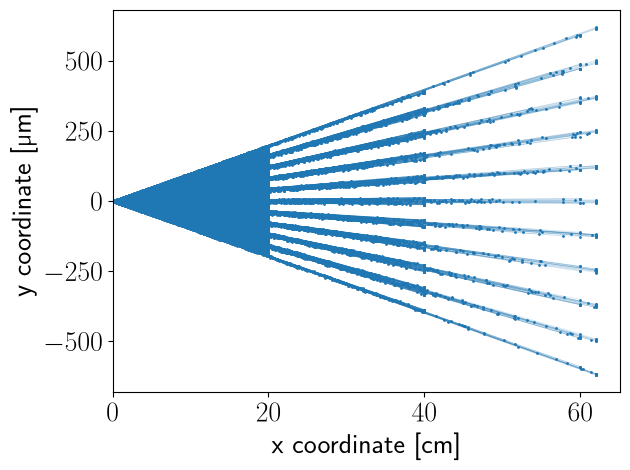
\includegraphics[width=0.95\linewidth]{moire/moire_without_g.png}
        \caption{Without gravity (\(a=0\))}
        \label{fig:moire-without-gravity}
    \end{subfigure}%
    \hfill
    \begin{subfigure}[t]{0.49\textwidth}
        \centering
        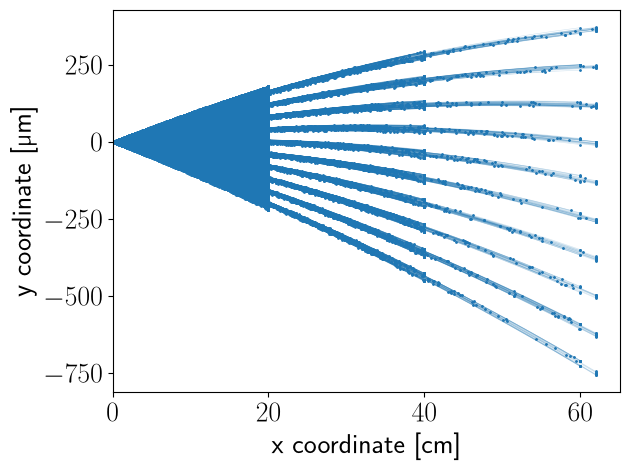
\includegraphics[width=0.95\linewidth]{moire/moire_with_g.png}
        \caption{With gravity (\(a=10^6g\))}
        \label{fig:moire-with-gravity}
    \end{subfigure}
    \caption[Moir\'e: simulated annihilation positions with and without gravity]{Illustration of the tracking of individual positronium atoms (shown as blue points) for the simulation parameters: \(v=10^5\) \si{\metre\per\second}, \(N=40\,000\), \(\theta=2\) mrad, \(L=20\) cm. Each atom is tracked, its annihilation position is determined, and then its position relative to the gratings is stored (the gratings can be clearly seen in the plots as clusters of the annihilation points at \(x=20,40,60\) cm).
    In panel \ref{fig:moire-with-gravity}, the gravitational acceleration was increased to \(10^6\ g\) to make the deflection clearly visible. Note that \(x\)-axis is in centimeters, while \(y\)-axis is in micrometers.}
    \label{fig:moirewithg}
    
\end{figure}

The number of equally spaced positions of the third grating sampled over one grating period \(d\) is denoted by \(N_{\mathrm{off}}\). The procedure is repeated independently at each position, with a step of \(d/N_{\mathrm{off}}\), and the atom count for each position is saved. Figure \ref{fig:moiresample} shows an example of the number of annihilations on the third grating, on the stopper, and in the space between them as a function of the third-grating position. The pattern shown in the figure is periodic with a period of \(d\); the plot shows only one period of the pattern.

\begin{figure}[ht!]
    \centering
    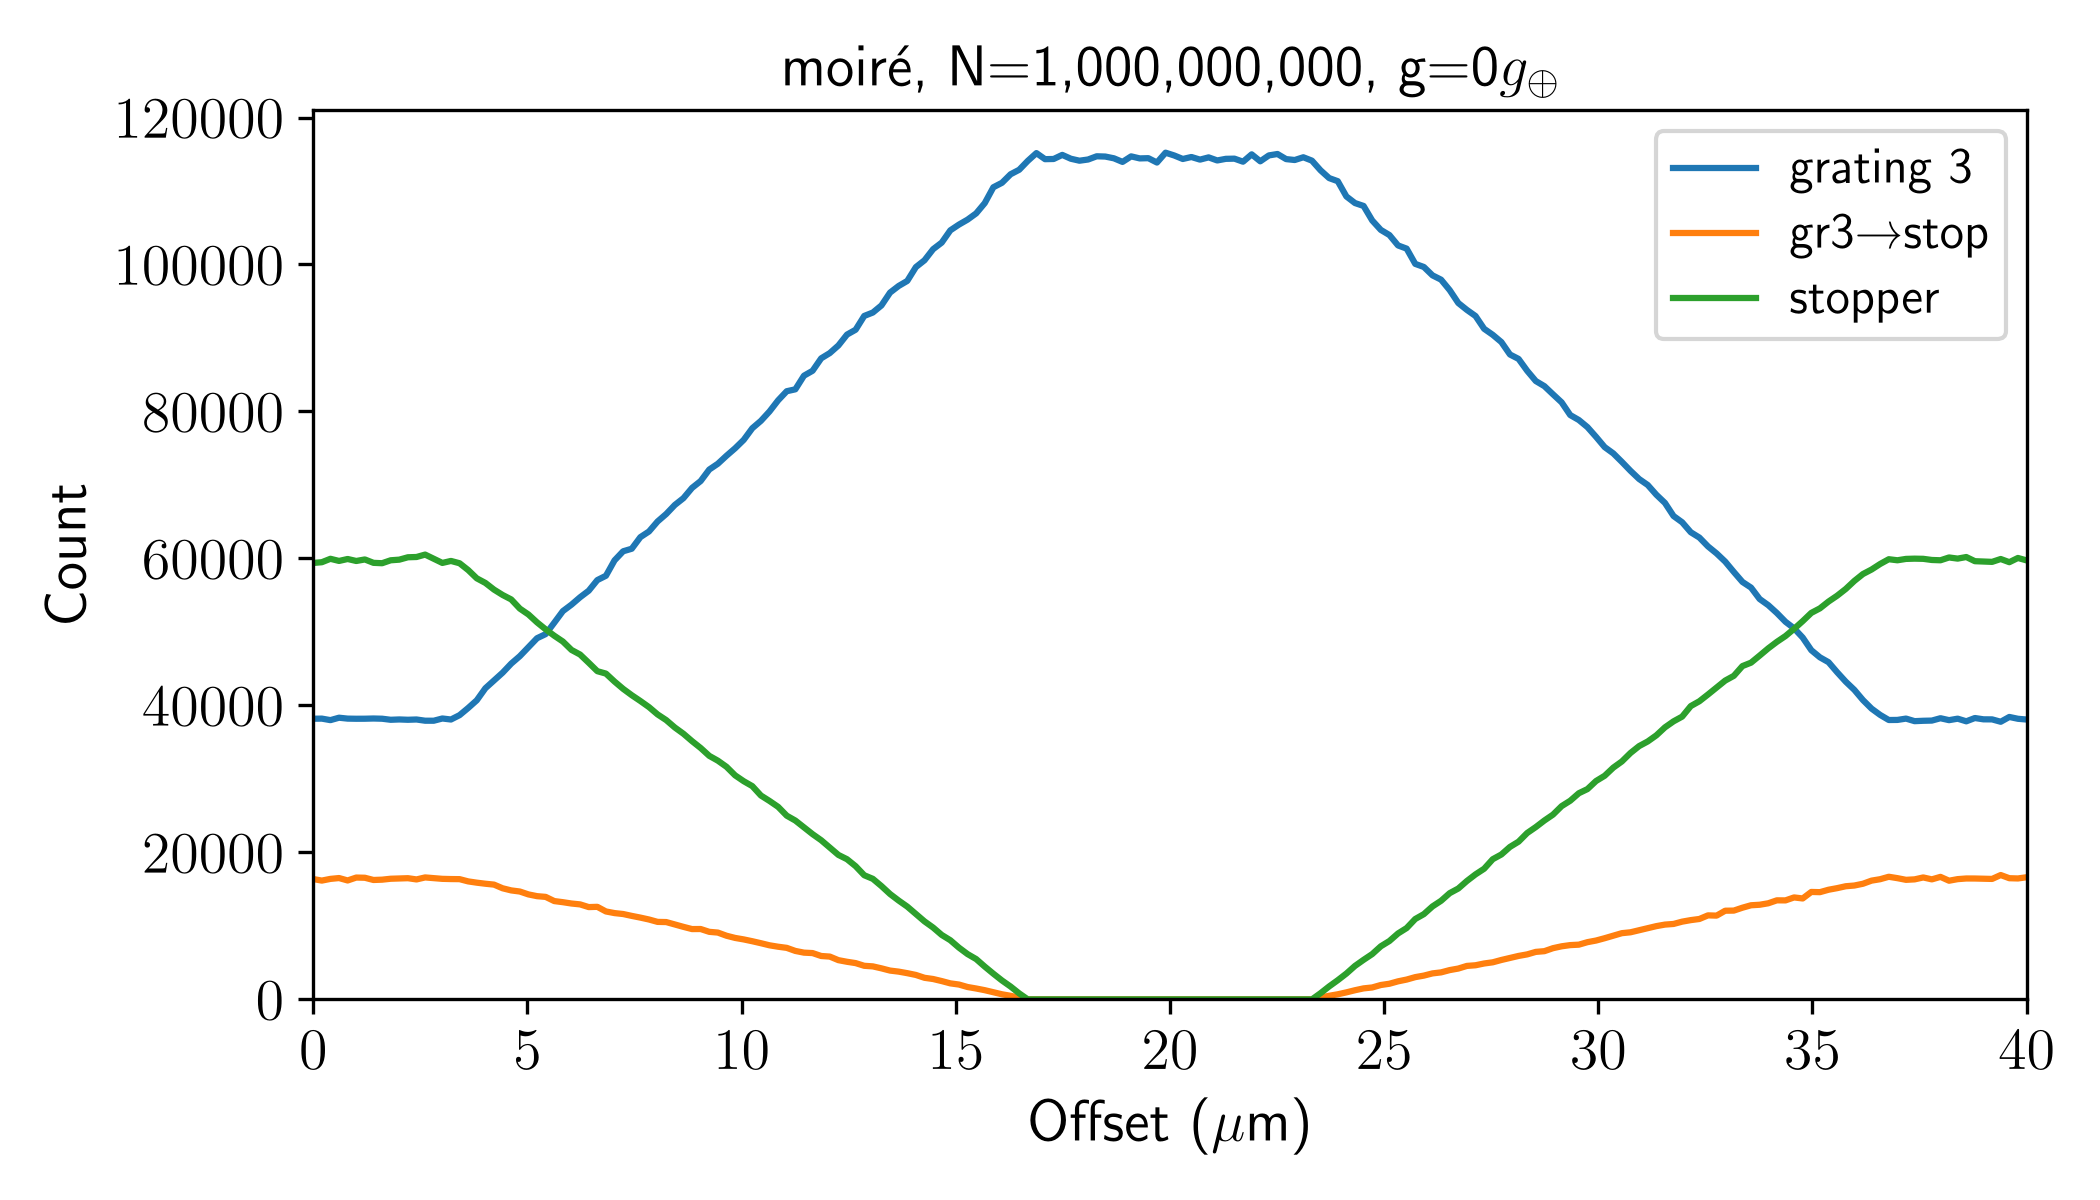
\includegraphics[width=0.75\textwidth]{moire/moirepattern.png}
    \caption[Moir\'e: annihilation counts versus third-grating position]{A plot of the annihilation count on the third grating (blue), on the stopper (green), and in the space between them (yellow) as a function of the position of the third grating \(y_3\), for the simulation parameters:  \(v=5\times10^4\) \si{\metre\per\second}, \(N=10^9\), \(\theta=5\) mrad, \(L=20\) cm. The count of the particles decaying or annihilating in other places is not shown, because they are outside the plotted range for the given parameters and are not physically meaningful (do not form a pattern). Approximately one in 8700 positronium atoms generated at the input reached the third grating.}
    \label{fig:moiresample}
    
\end{figure}

The shift of the moir\'e pattern in the presence of a force is shown in Figure \ref{fig:moire-inset}. Note that the accelerations used in this simulation were multiples of Earth's gravitational acceleration: since the minimum detectable acceleration by this method is given in~\cite{Mariazzi_Caravita_Doser_Nebbia_Brusa_2020} as \begin{equation}a_{\min}=\frac{d}{2\pi V t^2 \sqrt{N_{det}}},\label{eq:amin}\end{equation} where \(V\) is the visibility of the fringes, given by 
\begin{equation}
V=\frac{n_{max}-n_{min}}{n_{max}+n_{min}},
\label{eq:visibility}
\end{equation}\(n_{min}\) and \(n_{max}\) 
are the minimum and maximum values on the raw (unfitted) particle count on the stopper \(n(y_3)\) respectively, \(t=L/v\) is the interrogation time, and \(N_{det}\) is the number of detected atoms per scan, one can estimate that the detectability of the acceleration-based pattern shift scales with \(1/\sqrt{N_{in}}\), where \(N_{in}\) is the number of positronium atoms on input. In the case presented in the figure, it can be estimated that one can detect an acceleration of \(1g\) with this precision using 10,000 times as many particles.

\begin{figure}[ht!]
    \centering
    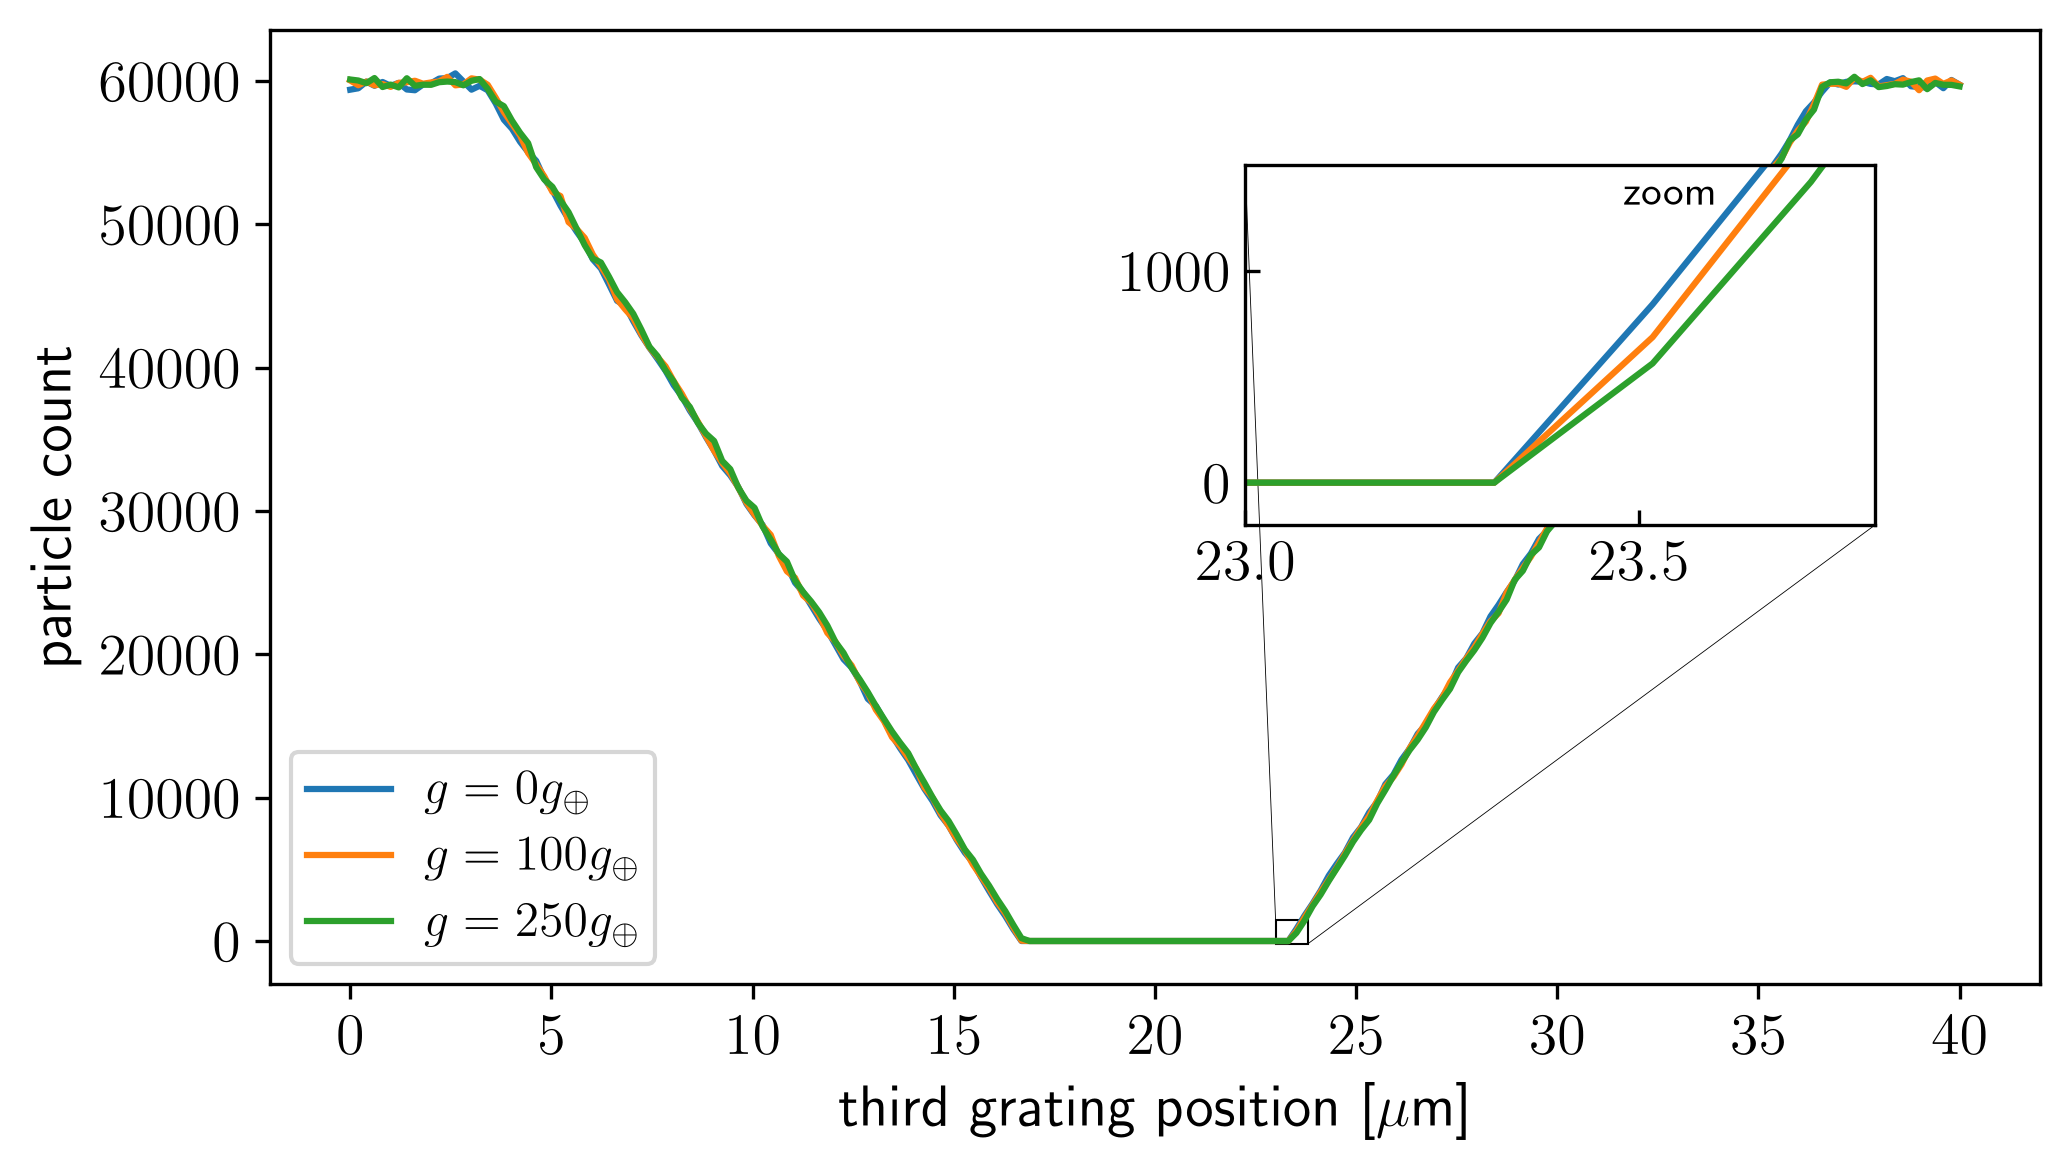
\includegraphics[width=0.8\textwidth]{moire/moire-inset.png}
    \caption[Moir\'e: gravity-induced pattern shift]{The particle count on the stopper as a function of the third-grating position for gravitational accelerations of \(0\), \(100g\), and \(250g\), where \(g\) denotes Earth's gravitational acceleration. The inset shows an enlarged view of the rising edge near the minimum, highlighting the differences between the three curves.}
    \label{fig:moire-inset}
\end{figure}


Figure \ref{fig:moire-sensitivity} shows the dependence of the minimum detectable acceleration \(a_{\min}\) on the angular beam divergence \(\theta_{\max}\), given the initial velocity \(v_0=10^5\) \si{\metre\per\second}. The sensitivity of the deflectometer increases with \(\theta_{\max}\), because the number of positronium atoms increases with the collimation angle (the positronium source emits atoms isotropically, and then the slit cuts out the uncollimated part of the beam). In the case of the moir\'e deflectometer, there is no global minimum of the minimum detectable acceleration, although there are limitations concerning the maximum reasonable beam divergence. Assuming a maximum angular divergence based on the article~\cite{Mariazzi_Caravita_Doser_Nebbia_Brusa_2020} -- \(\theta_{\max}=17\) mrad -- the minimum achievable detectable acceleration is equal to \((3408\pm31)\)~\si{\metre\per\second\squared}.

\begin{figure}[ht!]
    \centering
    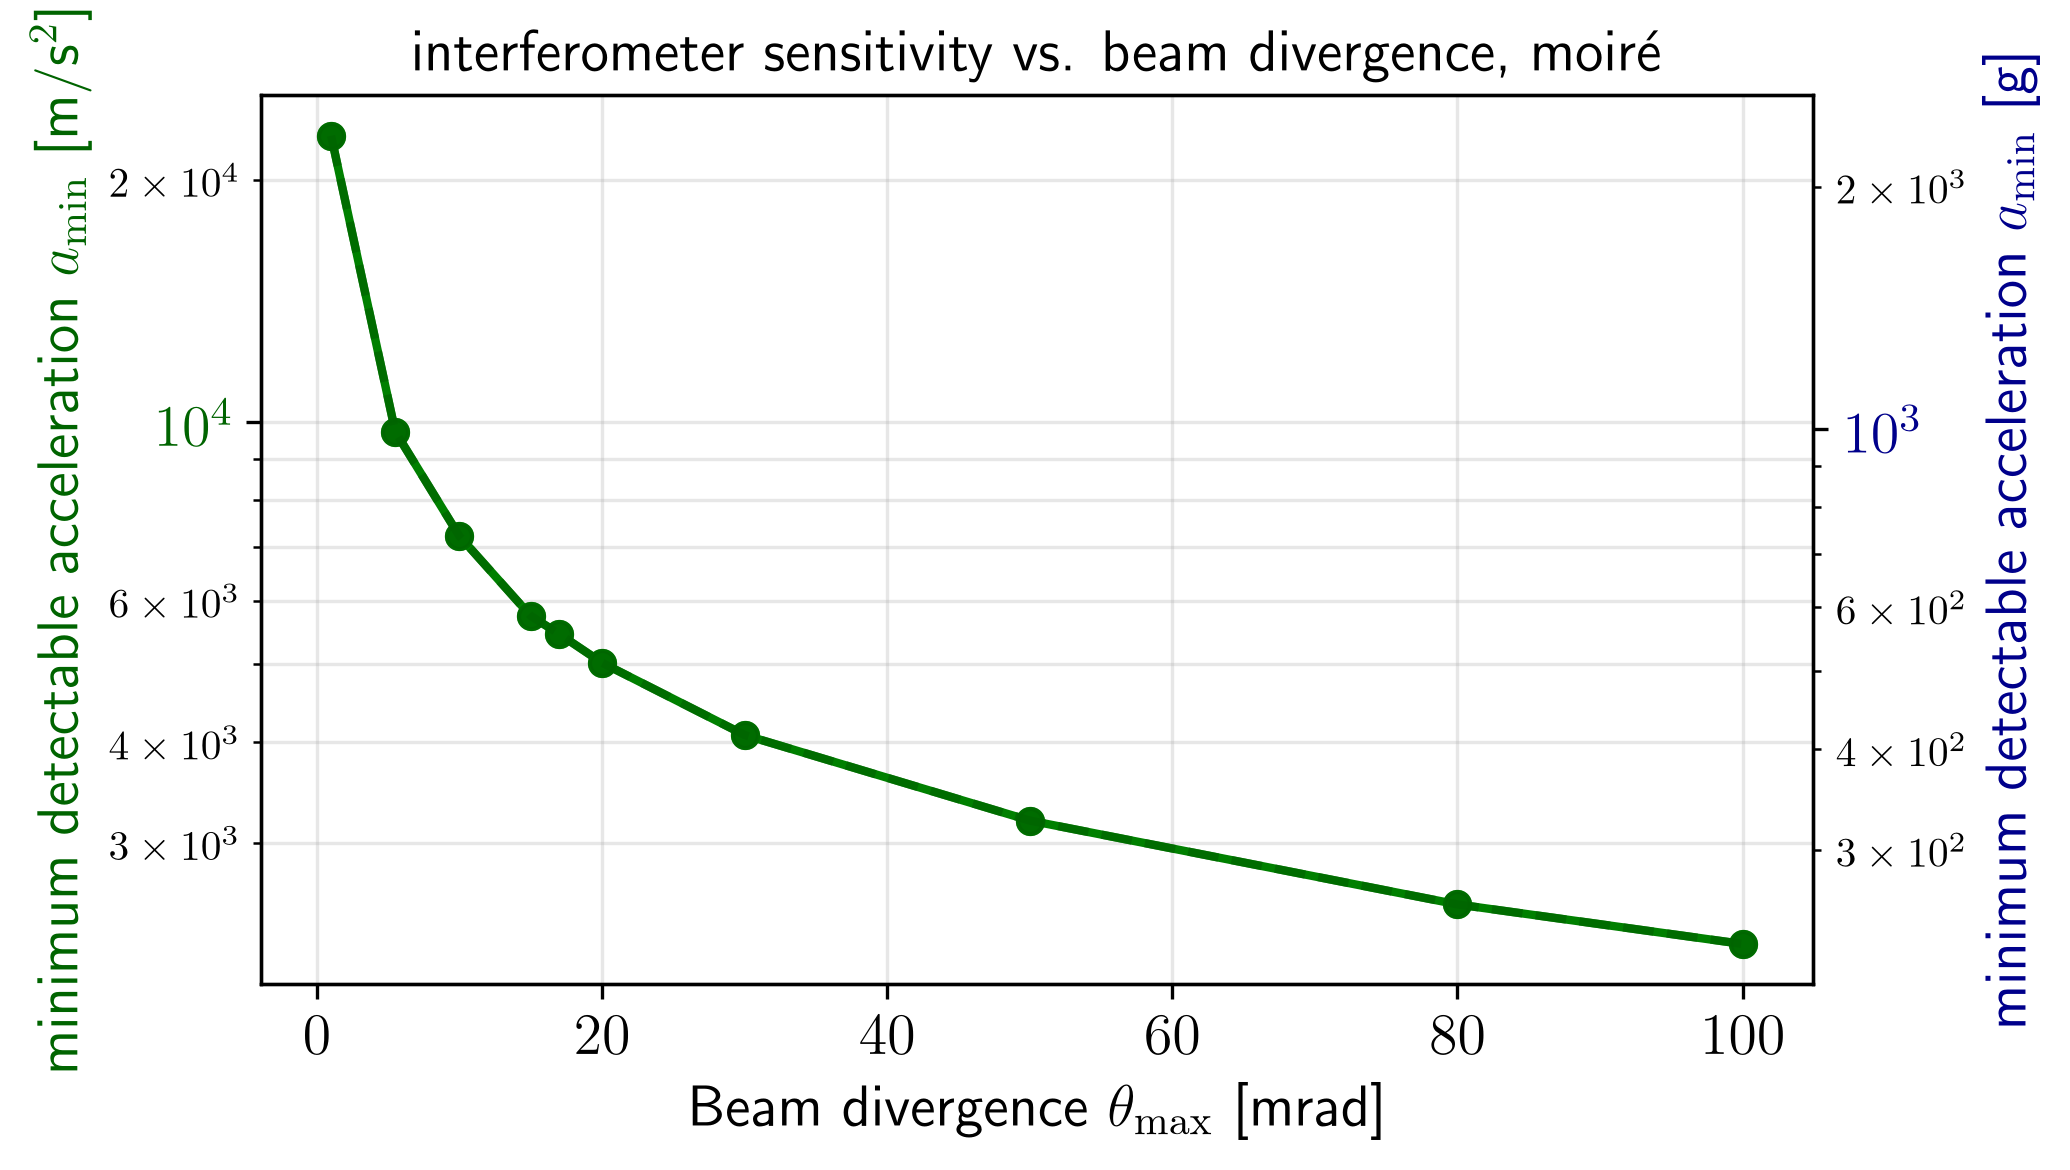
\includegraphics[width=0.85\textwidth]{moire/moire-sens.png}
    \caption[Moir\'e: sensitivity versus beam divergence]{The minimum detectable acceleration \(a_{\min}\) of the moir\'e deflectometer as a function of the beam divergence \(\theta_{\max}\). The left axis gives the acceleration in \si{\metre\per\second\squared}, while the right axis expresses it in units of Earth's gravitational acceleration \(g\).}
    \label{fig:moire-sensitivity}
\end{figure}

Figure \ref{fig:moire-amin-heatmap} shows a heatmap of the dependence of \(a_{\min}\) on the angular beam divergence \(\theta_{\max}\) (on the \(x\)-axis) and the mean initial velocity \(v_0\) (on the \(y\)-axis). Given the constraints on angular divergence described in the previous paragraph, to optimise the function realistically, one can find a minimum for a fixed \(\theta_{\max}\). However, the situation is different for the initial velocity \(v_0\): the minimum is a trade-off between two effects -- faster atoms accumulate a smaller gravitational shift, thus the smaller the fringe shift, but also the less time it spends inside the apparatus, and thus the greater the survival probability of positronium atoms.
Under these conditions, the lowest achievable value of \(a_{\min}\) for a given number of input particles is \(a_{\min}=(3382\pm30)\) \si{\metre\per\second\squared} or \((344.9\pm3.1)\ g\), for \(v_0=0.9\times10^5\) \si{\metre\per\second}. The reported value is the mean of ten independent simulation runs, and the quoted uncertainty is the standard deviation of the results across these runs. This uncertainty quantifies only the statistical scatter between independent Monte Carlo runs. It does not include systematic contributions from grating alignment, beam and source properties, or detector response.

\begin{figure}[ht!]
    \centering
    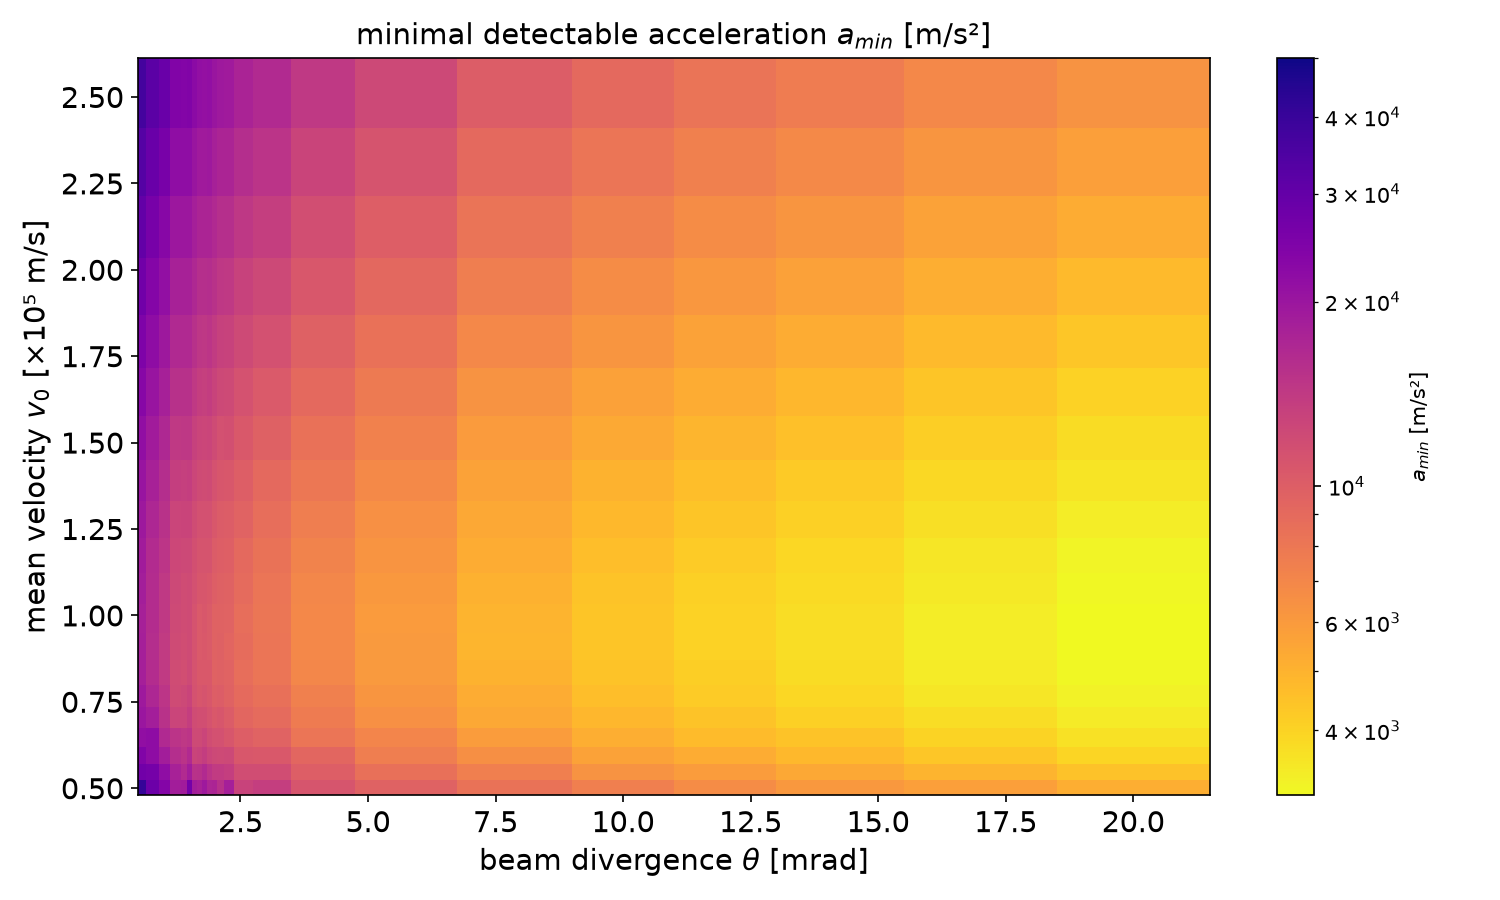
\includegraphics[width=0.85\textwidth]{moire/particles_amin_heatmap.png}
    \caption[Moir\'e: velocity--divergence sensitivity map]{The minimum detectable acceleration \(a_{\min}\) of the moir\'e deflectometer as a function of the beam divergence \(\theta_{\max}\) and the mean velocity \(v_0\). The colour scale indicates \(a_{\min}\) in \si{\metre\per\second\squared}.}
    \label{fig:moire-amin-heatmap}
\end{figure}

Knowing that sensitivity scales as \(1/\sqrt{N}\), to increase the sensitivity to \(g\), the experiment would have to run \((a_{\min}/g)^2\approx119\ 000\) times longer than in the simulated experiment (the number of shots \(N_s=400\)).


% \subsection{Geant4 simulation}

\section{Event-level Monte Carlo model of the Mach--Zehnder interferometer}

In the case of simulating the Mach--Zehnder interferometer, the main idea -- simulating a bunch of atoms, tracking each of them and saving its point of annihilation -- is the same as in the case of the moir\'e deflectometer. Also in this case, for each particle an initial velocity, an angle of incidence, and a lifetime are randomly assigned, as described in the previous section. 
In the underlying Mach--Zehnder interferometer, the positronium state evolves as a coherent superposition of the two paths.
During the flight between the first and second gratings, the total relative phase \(\phi_{total}\) accumulates, depending on the positions of the gratings and gravitational acceleration.
In this simulation, the total gravitational phase shift during the flight is given by 
\begin{equation}\phi=\frac{2\pi g t^2}{d},\end{equation} where \(t_=L/v\) is the time of flight (interrogation time), and a phase offset \(\phi_0=0\) is assumed (in a real experiment it is unknown, but constant, so this offset will be removed later). 
Then, the interference phase \(\theta\)  at the third, material grating is randomly chosen from \([0,2\pi)\) using rejection sampling with a probability density function determined by the Born rule (the probability that an atom will be found at a given vertical position): \begin{equation}\rho(\theta) = \frac{1}{2\pi}  \left(1 + C_{max} \cos(\theta + \phi)\right).\label{eq:interference-probability}\end{equation}
% where \(C_{max}\) is the maximum possible contrast (due to imperfect beam splitting in the gratings, it was set to \(C_{max}=0.8\)).
Here \(C_{\max}\) denotes the assumed intrinsic contrast of the interference pattern prior to the third grating’s readout. We assume \(C_{\max}=0.8\) in the present, purely phenomenological model. The Monte Carlo procedure only samples individual detection events from this density and propagates the effects of a finite lifetime, of a velocity spread, of an angular acceptance and of counting statistics to the reconstructed acceleration.

When the atom has its assigned interference phase \(\theta\), the algorithm simulates the action of the third grating: a periodic mask made of alternating bars and gaps with a period \(d\) and an open fraction \(f=0.5\). Its positional phase is defined as \begin{equation}\phi_y=\frac{2\pi y_3}{d}\mod2\pi.\end{equation} The algorithm then calculates the phase difference to determine whether an atom passes through the grating: \begin{equation}\begin{cases}
    (\theta-\phi_y)\mod 2\pi < 2\pi f & \text{atom passes}\\
    (\theta-\phi_y)\mod 2\pi \geq 2\pi f & \text{atom does not pass}.
\end{cases}\end{equation}

If the atom passes through the grating, its remaining lifetime is randomly chosen again (due to the memorylessness of the exponential distribution), and if the remaining lifetime is shorter than \(t_s=L_s/v\), the positronium atom annihilates in the gap between the third grating and the stopper; otherwise, it annihilates on the stopper. If the atom does not pass, its annihilation on the third grating is recorded.


\begin{figure}[ht!]
    \centering
    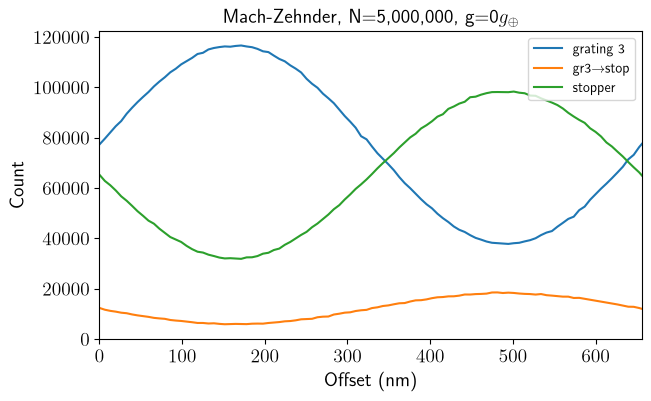
\includegraphics[width=0.8\textwidth]{mach/mach_zehnder_pattern.png}
    \caption[Mach--Zehnder: simulated annihilation counts]{Simulated annihilation counts on the third grating (blue), on the stopper (green), and in the gap between them (orange) as a function of the third-grating position \(y_3\) in the Mach--Zehnder interferometer, for \(N=5\times10^6\) and zero gravitational acceleration.}
    \label{fig:machsample}
\end{figure}

The entire procedure above is repeated for each atom at a given third grating position \(y_3\), and the total count of atoms annihilated on the third grating, annihilated on the stopper, or decaying in between is recorded. Then, the procedure is repeated for all positions in the distance of one period \(d\). Example simulation results are shown in Figure \ref{fig:machsample}.

\begin{figure}[ht!]
    \centering
    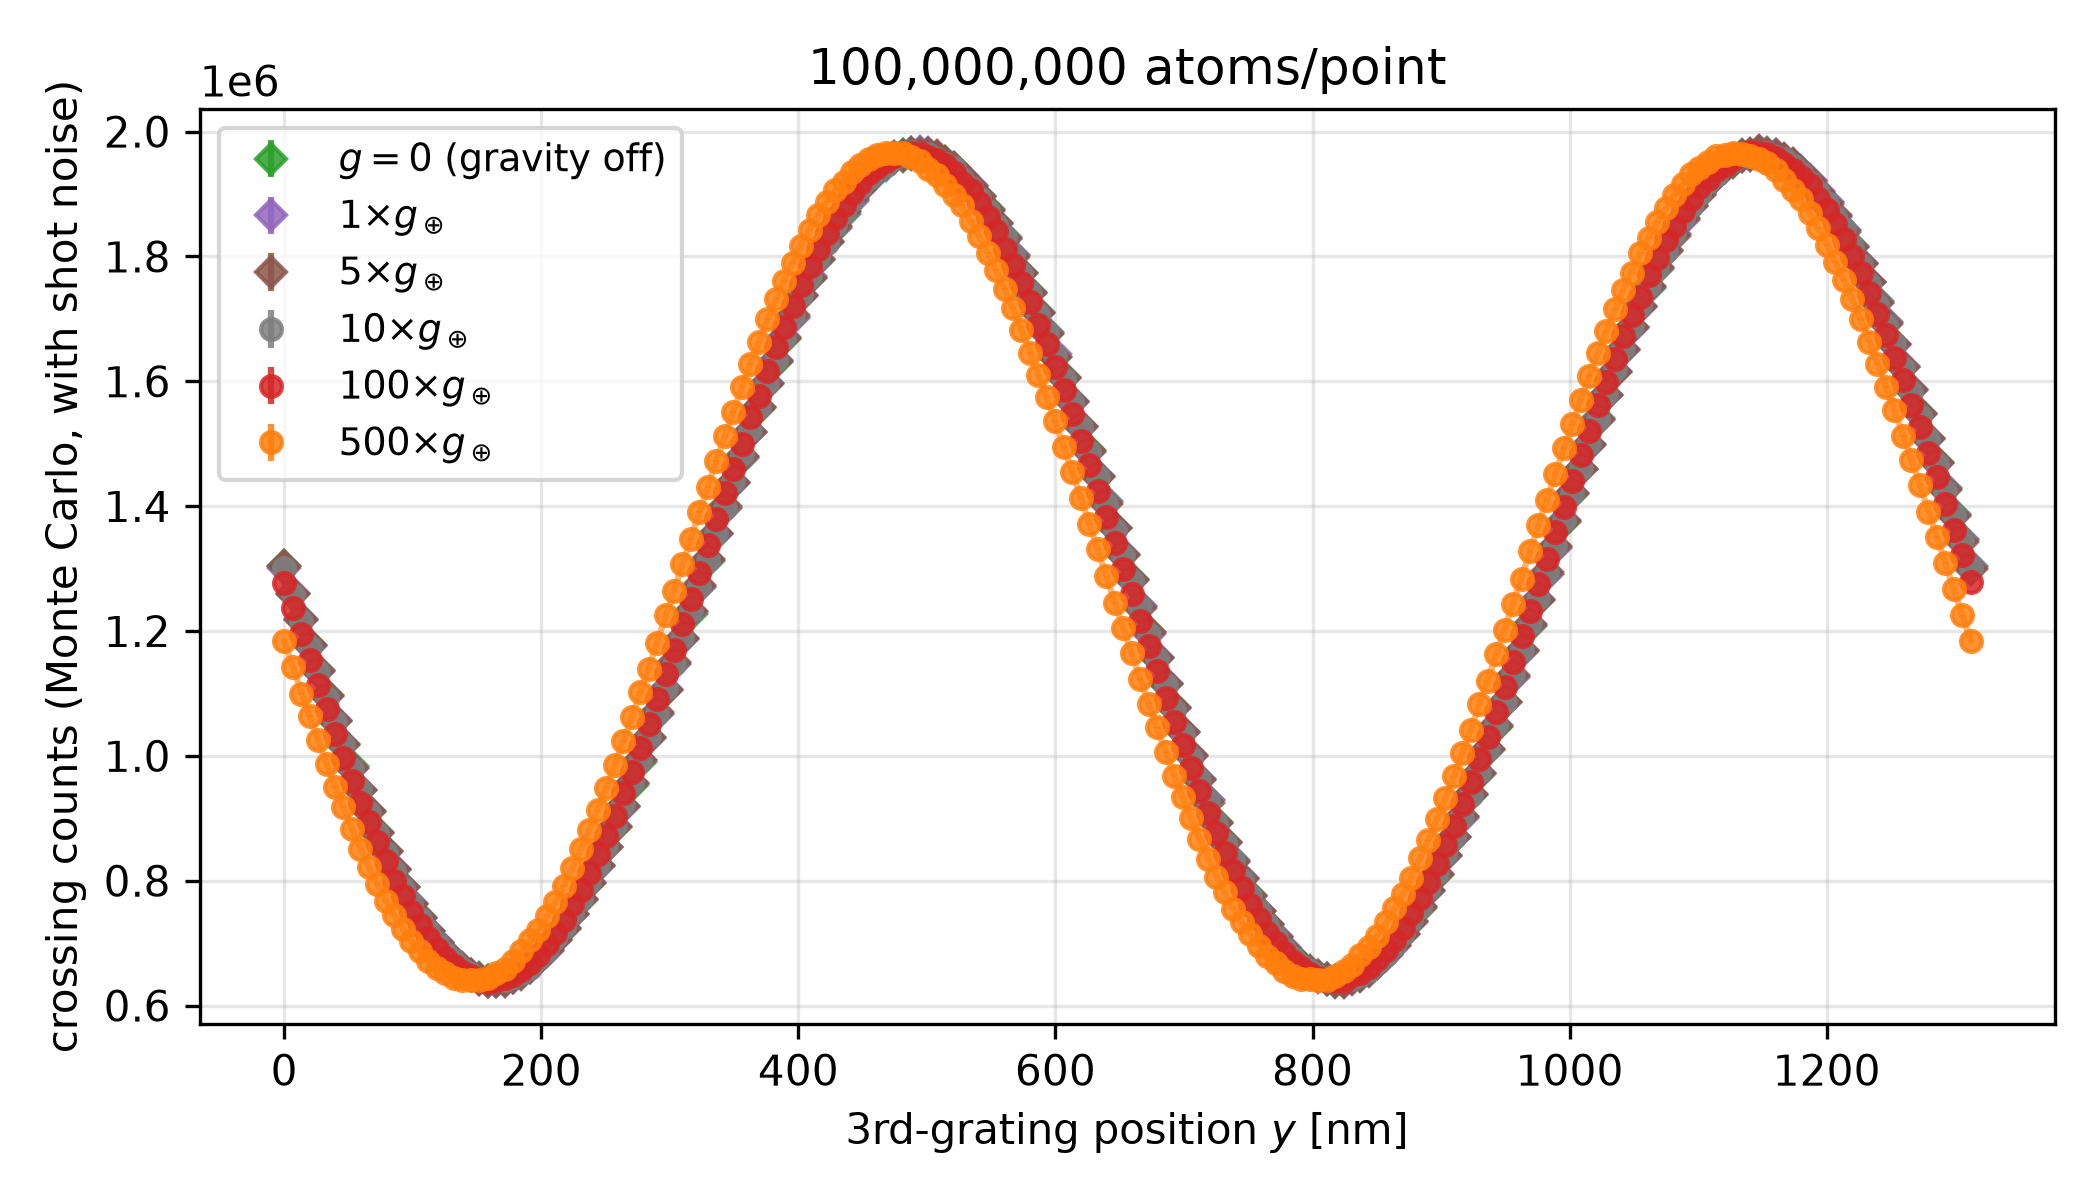
\includegraphics[width=0.9\textwidth]{mach/mariazzi_gravity_shift_mp.png}
    \caption[Mach--Zehnder: gravity-induced fringe shift]{Simulated counts of atoms passing through the third grating as a function of the position of the third grating \(y_3\) for accelerations of \(0\), \(g\), \(5g\), \(10g\), \(100g\), and \(500g\), where \(g\) denotes Earth's gravitational acceleration. Each scan point uses \(10^8\) atoms.}
    \label{fig:mach-gravity-shift}
\end{figure}

The phase shift from Figure \ref{fig:mach-gravity-shift} can be determined quantitatively by fitting the following equation to the data: 
\begin{equation}
    N(y_3)=N_0[1+C\cos(2\pi y_3/d + \phi)].
        \label{eq:transmission-pattern}
\end{equation} 
Here \(C\) denotes the fitted modulation amplitude of the third-grating transmission curve and should be distinguished from the input intrinsic contrast \(C_{\max}\) in Eq.~\eqref{eq:interference-probability}; \(V\) in Eq.~\eqref{eq:visibility} denotes the visibility evaluated directly from the maximum and minimum stopper counts.
From the fitted phase \(\phi\) the gravitational acceleration \(g\) can be reconstructed using 
\begin{equation}
    g=\frac{\phi d}{2\pi\langle t^2\rangle},
        \label{eq:acceleration-reconstruction}
\end{equation} 
where \(\langle t^2 \rangle\) is the effective mean square time of interrogation (which is needed because the velocity is not the same for each positronium atom, and atoms with a higher velocity have a higher probability of survival). 


\begin{figure}[ht!]
    \centering
    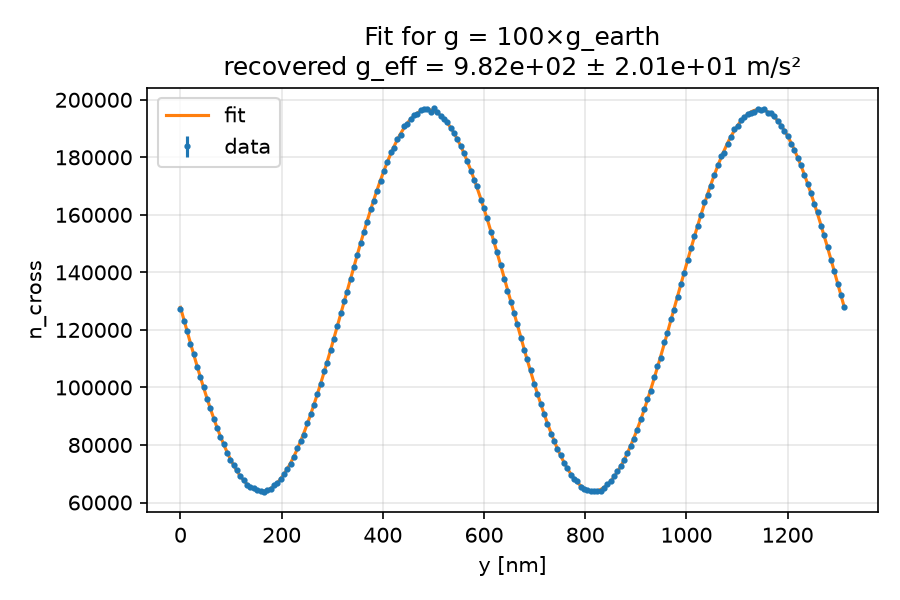
\includegraphics[width=0.9\textwidth]{mach/fit_100g_unwrapped.png}
    \caption[Mach--Zehnder: sinusoidal fit at \(100g\)]{Sinusoidal fit (orange line) to the simulated counts of atoms passing through the third grating (blue points) as a function of its position \(y_3\), for an applied acceleration of \(100g\). The acceleration reconstructed from the fitted phase is \((982 \pm 20.1)\)~\si{\metre\per\second\squared}, corresponding to \((100.1 \pm 2.1)g\), where \(g=9.81\)~\si{\metre\per\second\squared}. Each point on the plot corresponds to \(10^8\) positronium atoms generated at the input of the simulation.}
    \label{fig:mach-fit-100g}
\end{figure}

To compare the results of the simulation with previous calculations from the literature, we have to calculate the minimum detectable acceleration for 400 shots, i.e. 272\,000 positronium atoms per point on the interferometer input. To obtain \(a_{\min}\), we have to use Eq. \eqref{eq:amin} also in this case.

Figure \ref{fig:mach-sensitivity-divergence} shows \(a_{\min}\) as a function of the angular beam divergence \(\theta_{\max}\) for a fixed initial velocity \(v_0=10^5\) \si{\metre\per\second}. In contrast to the case of the moir\'e deflectometer (Figure \ref{fig:moire-sensitivity}), this plot shows a minimum in \(a_{\min}\) -- for a beam divergence of \(\theta_{\max}\approx1.6\) mrad, \(a_{\min}=(140\pm1)\) \si{\metre\per\second\squared} (averaged over 10 runs). This is due to the trade-off between two effects: an increase in the number of atoms and a decrease in visibility. On the one hand, as the beam divergence increases, the number of positronium atoms increases (\(N_0\propto \theta_{\max}\)). On the other hand, the Mach--Zehnder interferometer is very sensitive to angular coherence of the beam -- optical gratings accept only atoms with a finite acceptance angle~\cite{Dürr_Rempe_1999}, and in the simulation the acceptance is modelled using a Gaussian approximation 
\begin{equation}
    c_{atom}\propto \exp\left(\frac{-\theta_{in}^2}{2\sigma_{\mathrm{acc}}^2}\right),
    \label{eq:bragg-acceptance}
\end{equation} %where \(\theta_{in}\) is the angle of incidence, and \(\sigma_{\mathrm{acc}}\) is the Bragg acceptance angle (for an optical grating with \(\lambda=1312\) nm, \(\sigma_{\mathrm{acc}}\approx5.5\) mrad; see Eq. (6) in \cite{Mariazzi_Caravita_Doser_Nebbia_Brusa_2020}).
where \(\theta_{\rm in}\) is the angle of incidence and \(\sigma_{\rm acc}\) is a phenomenological width parameter describing the finite angular acceptance in the present simulation. For a standing-wave wavelength of \(\lambda=1312\)~nm, Ref.~\cite{Mariazzi_Caravita_Doser_Nebbia_Brusa_2020} obtains the diffraction angle
\[ 2\theta_B=\frac{\lambda_{\rm dB}}{d}\simeq5.5~\mathrm{mrad}, \]
from Eq.~(6), and uses this angle as a characteristic scale for the required angular collimation of the positronium beam. The value \(\sigma_{\rm acc}=5.5\)~mrad is therefore adopted here as the width of the Gaussian acceptance model. This Gaussian form should not be interpreted as the exact Bragg-reflection probability or as an expression derived in Ref.~\cite{Mariazzi_Caravita_Doser_Nebbia_Brusa_2020}. 
The actual angular dependence of Bragg reflection can be more complex within the finite acceptance region~\cite{Dürr_Rempe_1999}.

\begin{figure}[ht!]
    \centering
    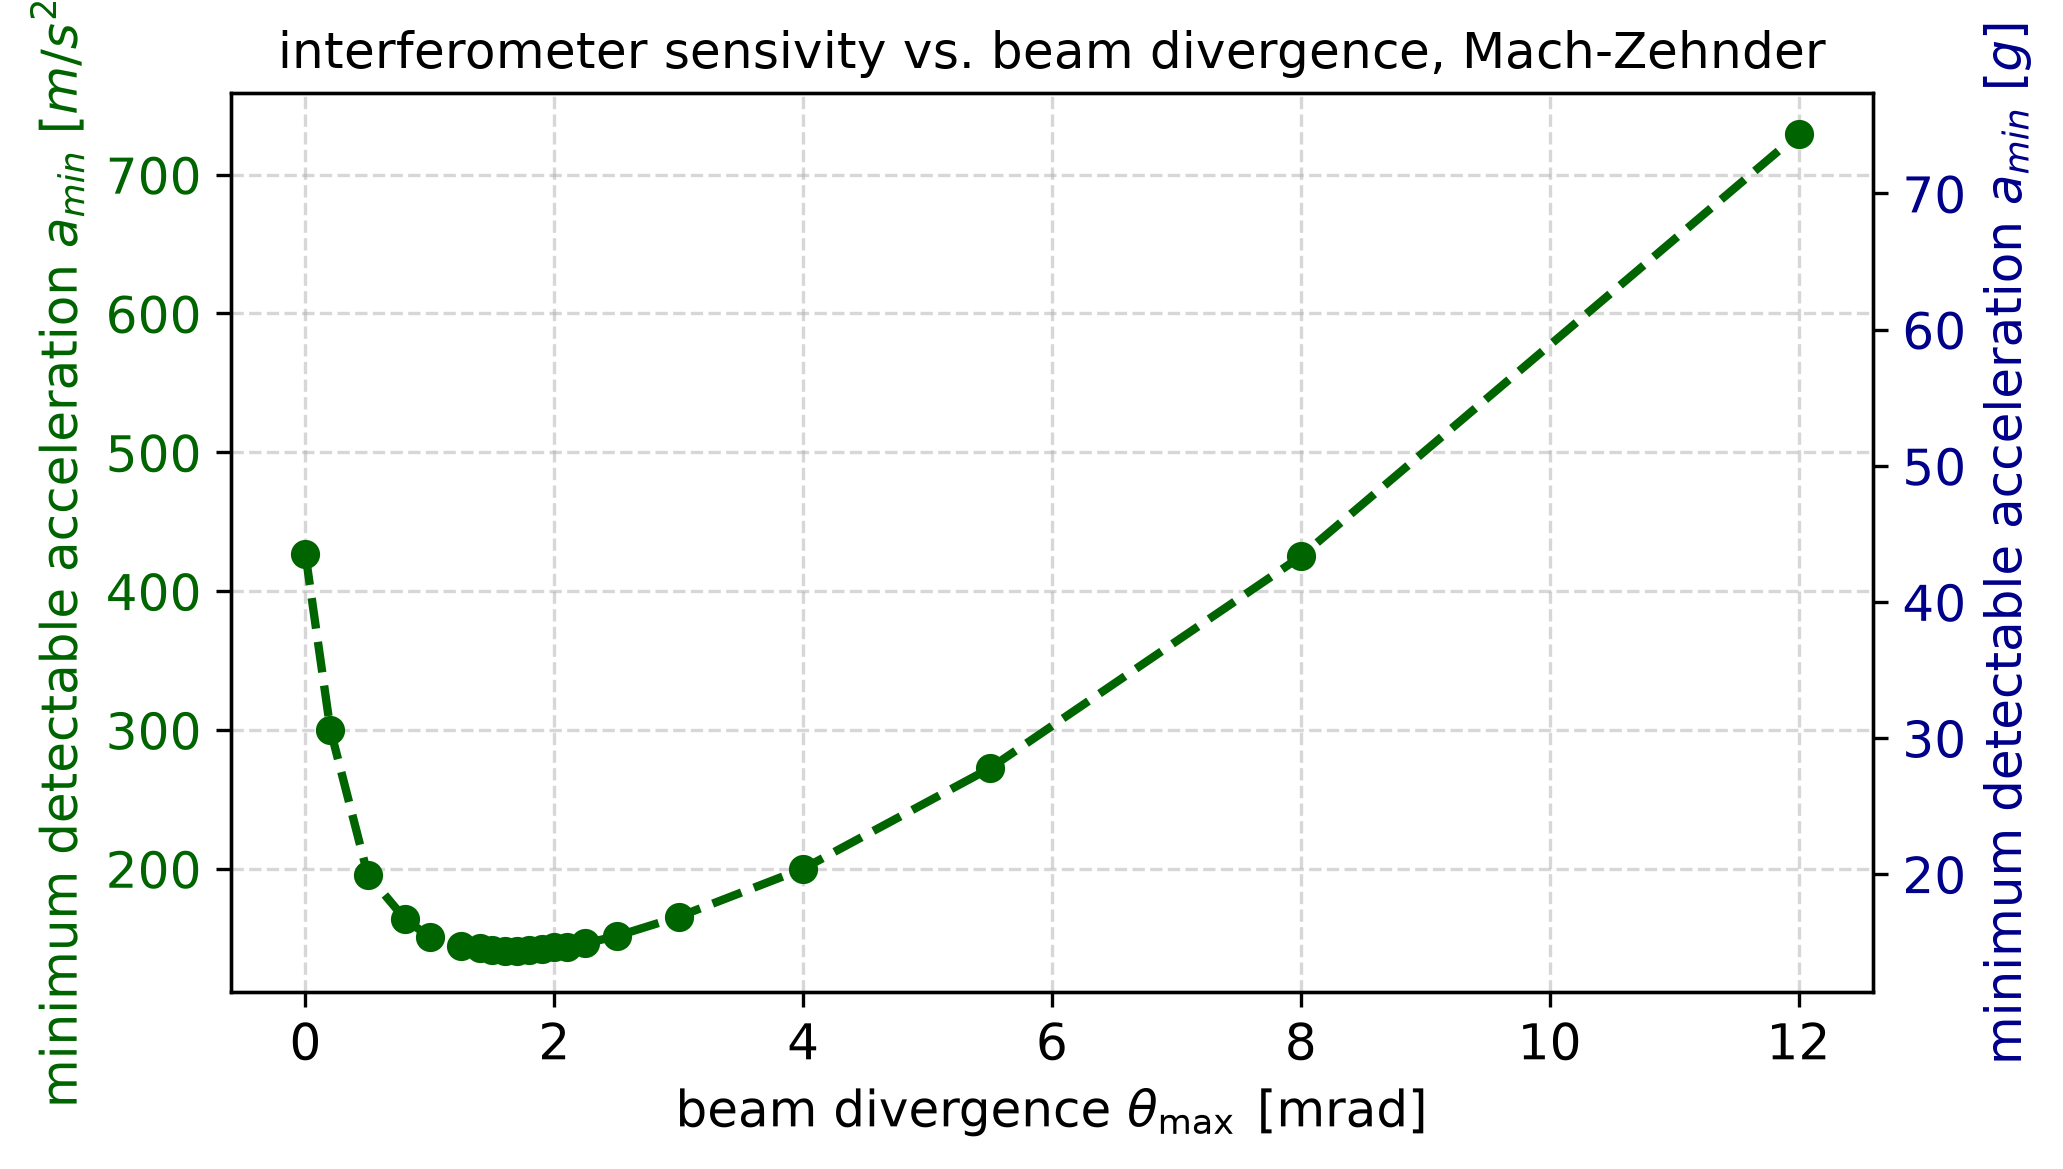
\includegraphics[width=0.8\textwidth]{mach/mz_sensitivity_vs_divergence_dual_axis.png}
    \caption[Mach--Zehnder: sensitivity versus beam divergence]{The minimum detectable acceleration \(a_{\min}\) of the Mach--Zehnder interferometer as a function of the beam divergence \(\theta_{\max}\). The left axis gives the acceleration in \si{\metre\per\second\squared}, while the right axis expresses it in units of Earth's gravitational acceleration \(g\).}
    \label{fig:mach-sensitivity-divergence}
\end{figure}

Figure \ref{fig:mach-amin-heatmap} shows a heatmap of
the minimum detectable acceleration as a function of the angular beam divergence \(\theta_{\max}\) and the mean initial velocity \(v_0\), showing a minimum at \(\theta_{\max}\approx1.6\) mrad and \(v_0\approx0.8\times10^5\) \si{\metre\per\second}. For these parameters, the minimum detectable acceleration is
\(a_{\min}=(134.6\pm1.2)\)~\si{\metre\per\second\squared}. The optimal region on the velocity-divergence plane is broad, so the experiment is highly tolerant of the exact choice of initial velocity and angular collimation -- these parameters can deviate by tens of per cent without significantly degrading the sensitivity.

\begin{figure}[ht!]
    \centering
    
\includegraphics[width=0.8\textwidth]{mach/parallel_amin_heatmap.png}
    \caption[Mach--Zehnder: velocity--divergence sensitivity map]{heatmap of the minimum detectable acceleration \(a_{\min}\) of the Mach--Zehnder interferometer as a function of beam divergence \(\theta_{\max}\) and mean velocity \(v_0\). The colour scale indicates \(a_{\min}\) in \si{\metre\per\second\squared}.}
    \label{fig:mach-amin-heatmap}
\end{figure}

\section{Comparative sensitivity analysis}

Table \ref{tab:method-comparison} summarises the sensitivity estimates for both methods: moir\'e deflectometry and Mach--Zehnder interferometry. For the simulated configurations with a fixed mean initial velocity \(v_0=10^5\) \si{\metre\per\second}, the Mach--Zehnder interferometer yields a minimum detectable acceleration lower by a factor of approximately 24 than that of the moir\'e deflectometer, which corresponds to a 593-fold shorter time of experiment, for the same detectable acceleration (since \(N\propto1/a_{\min}^2\)).

To compare the simulations with the literature estimates from~\cite{Mariazzi_Caravita_Doser_Nebbia_Brusa_2020}, the estimated values must be rescaled to the same total number of shots as in the simulation. The simulations used \(N_b=400\) shots per scan point with \(N_{\mathrm{off}}=200\) scan points, whereas the values in~\cite{Mariazzi_Caravita_Doser_Nebbia_Brusa_2020} correspond to approximately 400 shots of positronium atoms in total, for an entire scan. Since \(a_{\min}\propto1/\sqrt{N}\), the literature values are divided by \(\sqrt{N_{\mathrm{off}}}=\sqrt{200}\approx14.1\).

Table~\ref{tab:method-comparison} is not a point-by-point check of identical calculations. The two calculations summarized in the table have different statistics and different treatments of several important quantities, including the angular acceptance, fringe contrast, and the velocity distribution.% The values from the literature have only been scaled by a factor to ensure that the calculations have been performed for the same total number of shots, i.e. $N_b N_{\mathrm{off}}$. 
The remaining differences in physical assumptions are retained and discussed below.

\begin{table}[ht!]
    \centering
    \caption[Sensitivity comparison: simulations and literature]{Comparison of the minimum detectable accelerations \(a_{\min}\) obtained in the simulations and reported in the literature for a mean initial velocity of \(v_0=10^5\)~\si{\metre\per\second}. The simulations use 400 shots per scan point, while the literature estimates correspond to approximately 400 shots (Table 2 in~\cite{Mariazzi_Caravita_Doser_Nebbia_Brusa_2020}). The beam divergences used in each case are listed in the table. Here, \(g=9.81\)~\si{\metre\per\second\squared}.}
    \label{tab:method-comparison}
    \small
    \setlength{\tabcolsep}{4pt}
    \begin{tabular*}{\textwidth}{@{\extracolsep{\fill}}lccc@{}}
        \toprule
        Source & \(\theta_{\max}\) [mrad] & \(a_{\min}\) [\si{\metre\per\second\squared}] & \(a_{\min}/g\) \\
        \midrule
        \multicolumn{4}{@{}l}{\textbf{moir\'e}} \\
        Simulation & \(17\) & \(3408\pm31\) & \(347.4\pm3.2\) \\
        Literature & \(17\) & \(\sim 4.25\times10^3\) & \(\sim 4.3\times10^2\) \\
        \addlinespace
        \multicolumn{4}{@{}l}{\textbf{Mach--Zehnder}} \\
        Simulation & \(1.6\) & \(140\pm1\) & \(14.27\pm0.10\) \\
        Literature & \(5.5\) & \(\sim 6.9\times10^1\) & \(\sim 7.1\) \\
        \bottomrule
    \end{tabular*}
\end{table}

After rescaling the literature values to the simulation statistics of total number of shots \(N_bN_{\mathrm{off}}=8\times10^4\), the moir\'e deflectometer result agrees with literature to within \(\sim25\%\), while for the Mach--Zehnder interferometer the simulation predicts a sensitivity about two times worse than~\cite{Mariazzi_Caravita_Doser_Nebbia_Brusa_2020}, i.e. the simulated \(a_{\min}\) is a factor of \(\sim2\) larger than the rescaled literature value. 
The remaining factor of about two could originate from the different treatment of the angular acceptance, fringe contrast and the velocity averaging. Since they are varied simultaneously, their individual effects cannot be separated here; doing so would be useful in future work.
However, both the simulations and the literature estimates confirm the advantage of Mach--Zehnder interferometry over the moir\'e deflectometry for the same measurement time.


\chapter{Conclusions}
The main objective of this thesis has been to compare the sensitivity of two different inertial-sensing schemes, i.e. a classical moir\'e deflectometer and a Mach--Zehnder interferometer, by means of Monte Carlo simulation. For this purpose both devices have been modelled at single-atom level. Thus the atoms were propagated with velocities chosen from distribution based on measured $2^3S$ beam characteristics, a given angular spread and a lifetime chosen exponentially from an appropriate distribution with mean-lifetime of 1142 ns. 
The gravitational acceleration has then been reconstructed from the displacement (deflectometer) or the fitted phase (interferometer) of the transmission pattern [Eqs.~\eqref{eq:transmission-pattern} and~\eqref{eq:acceleration-reconstruction}]. The reconstructed value has been compared with the input value and found to be unbiased within the given statistics for a value of applied acceleration of $100g$ (Fig.~\ref{fig:mach-fit-100g}).

For a mean velocity of $v_0 = 10^5~\mathrm{m/s}$ and $3.2\times10^6$ s $\approx5.3$ weeks of acquisition time we find for the Mach--Zehnder interferometer a minimum detectable acceleration of $(140 \pm 1)~\mathrm{m/s^2}$ $\,(14.27 \pm 0.10\,g)$ at a beam divergence of $\theta_{\max} \approx 1.6~\mathrm{mrad}$ (Figure~\ref{fig:mach-sensitivity-divergence}). 
For comparison, at a beam divergence of \(\theta_{\max}=17\)~mrad, adopted from Ref.~\cite{Mariazzi_Caravita_Doser_Nebbia_Brusa_2020} the moir\'e deflectometer yields \(a_{\min}=(3408\pm31)\)~\si{\metre\per\second\squared}, corresponding to \((347.4\pm3.2)g\) (Figure~\ref{fig:moire-sensitivity} and Table~\ref{tab:method-comparison}).
% In contrast to this the moir\'e deflectometer reaches a minimum detectable acceleration of $(3408 \pm 31)~\mathrm{m/s^2}$ $\,(347.4 \pm 3.2\,g)$ at a beam divergence of $\theta_{\max} = 17~\mathrm{mrad}$ (Figure~\ref{fig:moire-sensitivity} and Table~\ref{tab:method-comparison}). 
Hence the interferometer is about $24$ times more sensitive than the moir\'e deflectometer, in order-of-magnitude agreement with the analytical estimate of Ref.~\cite{Mariazzi_Caravita_Doser_Nebbia_Brusa_2020}, which gives a ratio of several tens. The required number of atoms for a given target acceleration $a$ scales as $a_{\min}^{-2}$. Thus the measurement time for the Mach--Zehnder interferometer is about $593$ times shorter than for the moir\'e deflectometer.

An important distinction between the two instruments is how the sensitivity of the instrument depends on the beam. For the moir\'e deflectometer, the minimum detectable acceleration decreases monotonically with divergence (Fig.~\ref{fig:moire-sensitivity}). The maximum number of atoms that pass through the collimation slit increases linearly with the collimation angle $\theta_{\max}$. The limiting factor is then the angular acceptance of the two gratings. For the Mach--Zehnder interferometer, there is an optimum value for the maximum divergence of the atoms, $\theta_{\max} \approx 1.6~\mathrm{mrad}$ (Fig.~\ref{fig:mach-sensitivity-divergence}). 
% \sout{At this value, the number of atoms that pass through the interferometer grows with the square of the slit width, while the visibility of the fringes decreases as the slit width is increased beyond this value, due to the atoms having a divergence that is larger than the Bragg acceptance angle.}
For larger accepted angular divergences, the number of positronium atoms entering the interferometer increases approximately linearly in the present beam model. However, the reconstructed fringe visibility decreases with increasing divergence because atoms at larger incidence angles contribute less effectively to the interferometric signal due to the finite angular acceptance of the optical gratings.
This is expressed in Eq.~\eqref{eq:bragg-acceptance}~\cite{Dürr_Rempe_1999}. The two-dimensional plot of the sensitivity for the interferometer (Fig.~\ref{fig:mach-amin-heatmap}) clearly shows that this optimum is shallow. That is, near the minimum, the interferometer has a tolerance of several tens of percent in both velocity and divergence without a significant loss in sensitivity. This is an important property for a real apparatus, as it means that there is some flexibility in the preparation of the beam.

% The absolute sensitivities obtained here are lower than the analytical values of Ref.~\cite{Mariazzi_Caravita_Doser_Nebbia_Brusa_2020} by a factor of about $18$ for the moir\'e deflectometer and about $7$ for the Mach--Zehnder interferometer (Table~\ref{tab:method-comparison}). This difference should not be interpreted as an actual improvement in the performance of the devices, since it results mainly from different assumptions in the two calculations. Several differences in the assumptions contribute to this discrepancy. First, the time for interrogation, $t$, is evaluated by Ref.~\cite{Mariazzi_Caravita_Doser_Nebbia_Brusa_2020} as $L/v$, the time for an atom to travel between the slits of adjacent gratings. As noted above, this is the physical time to measure, and so differs from the above estimate for the transit time of an atom through the interferometer. Note that $a_{\min}$ is proportional to the inverse square of $t$ [Eq.~\eqref{eq:amin}], and thus this difference is most important for the deflectometer. The simulation adopts a maximum interference contrast of $C_{\max}=0.8$, while the realized fringe visibility, defined by Eq.~\eqref{eq:visibility}, is approximately $V\approx0.5$. This is higher than the conservative value of $V=0.3$ assumed in Ref.~\cite{Mariazzi_Caravita_Doser_Nebbia_Brusa_2020}. Since $a_{\min}\propto V^{-1}$ [Eq.~\eqref{eq:amin}], this difference accounts for part of the more optimistic sensitivity obtained in the present simulation.
% 
The sensitivities obtained in the present simulations are compared with the analytical estimates of Ref.~\cite{Mariazzi_Caravita_Doser_Nebbia_Brusa_2020} in Table~\ref{tab:method-comparison}, normalised to the same total number of shots. For the moir\'e deflectometer the simulation reproduces the analytical estimate to within $\sim25\%$. For the Mach--Zehnder interferometer the simulated $a_{\min}$ is about a factor of $2$ larger, i.e.\ the simulation predicts a sensitivity about two times worse than the estimate in Ref.~\cite{Mariazzi_Caravita_Doser_Nebbia_Brusa_2020}. 
The remaining difference originates from the different angular acceptance, fringe contrast and velocity averaging in the two calculations. Since, the above-mentioned assumptions are all different from each other, a quantitative separation of their individual contributions to the discrepancy is not possible within the scope of this work.
%
The beam divergence of the interferometer has been estimated above as $1.6~\mathrm{mrad}$, whereas for the same configuration Ref.~\cite{Mariazzi_Caravita_Doser_Nebbia_Brusa_2020} stated a divergence of $5.5~\mathrm{mrad}$. The remaining difference between the two estimates is due to normalization of the above counts to the number of atoms in the interferometer. When the conventions of Ref.~\cite{Mariazzi_Caravita_Doser_Nebbia_Brusa_2020} are applied consistently to both devices, the estimates agree, and the interferometer-to-deflectometer ratio is preserved, since a common interrogation time cancels in the ratio.

The interferometer result in the figure should be viewed as a statistical readout model of the interferometer rather than a full first-principles simulation of the interferometer of coherent positronium and laser. Thus, the sign and absolute value of $a_{\min}$ depend on the contrast and Bragg-acceptance parametrizations used in the model. %The main result is a comparison of the sensitivities and the identification of the velocity–divergence operating region in this model.

Two limitations should be stated here. First, the Mach--Zehnder interferometer is an intrinsically quantum device. A Geant4 cross-check was therefore not performed for the interferometer; for the classical deflectometer such a cross-check remains a useful validation and is left for future work. Second, the simulation does not include experimental systematic effects. The dominant ones for this scheme are the alignment and rotation of the gratings, the finite grating--stopper distance, and the pick-off annihilation of $2^3S$ atoms on the material elements, which affect the assignment of the annihilation position and the extracted contrast~\cite{Mariazzi_Caravita_Doser_Nebbia_Brusa_2020,Cooke2015}. The low polarizability of the $2^3S$ state limits its sensitivity to stray electric fields, which is one reason it is preferred over Rydberg states~\cite{Cassidy_2018,Mariazzi_Caravita_Doser_Nebbia_Brusa_2020}.

These results support the feasibility of further studies toward a first inertial measurement on a purely leptonic matter--antimatter system. No direct gravitational measurement on positronium yet exists~\cite{Bass_Mariazzi_Moskal_Stepien_2023,Mariazzi_Caravita_Doser_Nebbia_Brusa_2020}. The corresponding measurement on antihydrogen has only recently been reported~\cite{Anderson_etal_2023}. The moir\'e technique is under development for antihydrogen within AEgIS~\cite{Ferguson_AEḡISCollaboration_2025}. For weak accelerations, the interferometer is preferred because its standing-wave gratings are almost fully transparent, so few atoms are lost, and its period is short~\cite{Mariazzi_Caravita_Doser_Nebbia_Brusa_2020,Oberthaler_2002}. Reaching an acceleration of order $10\,g$ would require only a modest increase in the number of shots, compared to the simulated statistics. The gravitational regime relevant to a test of the weak equivalence principle needs far more integration time, or a larger usable flux. Ref.~\cite{Mariazzi_Caravita_Doser_Nebbia_Brusa_2020} identifies two routes to the latter: two-dimensional laser Doppler cooling to reduce the beam divergence, and coherent Raman excitation of the $2^3S$ level to raise its production. The broad optimum found here shows that these steps need no stringent re-optimization of the beam. With the position-sensitive detection under development for this purpose~\cite{Sharma_Baran_Brusa_Caravita_Chug_Coussat_Curceanu_Czerwiński_Dadgar_Dulski_etal._2023,Sharma_Povolo_Mariazzi_Korcyl_Kacprzak_Kumar_Niedźwiecki_Baran_Beyene_Brusa_etal._2024}, a first test of the free fall of positronium becomes a realistic longer-term goal.

\clearpage
\thispagestyle{numberonly}

\section*{Declaration of artificial intelligence and information technologies usage in the process of thesis writing}
\addcontentsline{toc}{section}{Declaration of artificial intelligence and information technologies usage in the process of thesis writing}

I declare the usage of the following generative AI tools in thesis writing and preparation:
\begin{itemize}
\item Deepseek V3, V4-flash \& R1: code generation and correction, literature checks, English grammar and vocabulary help, calculations verification
\item Claude Sonnet 4.6: code generation
\item Gemini 3.1 Pro, 3.5 Flash \& 3.6 Flash: code correction, literature search
\item Prism OpenAI Codex GPT-5.2: \LaTeX{} and Ti\emph{k}Z generation and correction, English grammar help
\item Duck.ai gpt-5.0, gpt-5.4-nano \& gpt-5.6-luna: answering my stupid programming questions
\end{itemize}

I wrote the thesis text myself, using AI tools for language correction and editorial assistance. No AI was used to generate the ideas or concepts of the thesis. After the usage of the listed tools I have verified and edited the content, and I take full responsibility for this publication.\todo{according to JU Rector's Ordnance 115/2025 on usage of tools based on artificial intelligence in didactics}

\section*{Acknowledgements}
\addcontentsline{toc}{section}{Acknowledgements}

I would like to thank my supervisor, dr Sushil Sharma, for his guidance and support throughout this work. I am grateful to Prof.\ dr hab.\ Paweł Moskal for the opportunity to carry out this research within the J-PET group at the Marian Smoluchowski Institute of Physics, Jagiellonian University. This work was supported by the National Science Centre, Poland (Narodowe Centrum Nauki), under grant No.\ 2023/50/E/ST2/00574 (SONATA BIS).


\printbibliography[heading=bibintoc]




\end{document}
